%  LaTeX support: latex@mdpi.com 
%  For support, please attach all files needed for compiling as well as the log file, and specify your operating system, LaTeX version, and LaTeX editor.

%=================================================================
\documentclass[sensors,article,accept,pdftex,moreauthors]{Definitions/mdpi} 
% For posting an early version of this manuscript as a preprint, you may use "preprints" as the journal and change "submit" to "accept". The document class line would be, e.g., \documentclass[preprints,article,accept,moreauthors,pdftex]{mdpi}. This is especially recommended for submission to arXiv, where line numbers should be removed before posting. For preprints.org, the editorial staff will make this change immediately prior to posting.

%--------------------
% Class Options:
%--------------------
%----------
% journal
%----------
% Choose between the following MDPI journals:
% acoustics, actuators, addictions, admsci, adolescents, aerospace, agriculture, agriengineering, agronomy, ai, algorithms, allergies, alloys, analytica, animals, antibiotics, antibodies, antioxidants, applbiosci, appliedchem, appliedmath, applmech, applmicrobiol, applnano, applsci, aquacj, architecture, arts, asc, asi, astronomy, atmosphere, atoms, audiolres, automation, axioms, bacteria, batteries, bdcc, behavsci, beverages, biochem, bioengineering, biologics, biology, biomass, biomechanics, biomed, biomedicines, biomedinformatics, biomimetics, biomolecules, biophysica, biosensors, biotech, birds, bloods, blsf, brainsci, breath, buildings, businesses, cancers, carbon, cardiogenetics, catalysts, cells, ceramics, challenges, chemengineering, chemistry, chemosensors, chemproc, children, chips, cimb, civileng, cleantechnol, climate, clinpract, clockssleep, cmd, coasts, coatings, colloids, colorants, commodities, compounds, computation, computers, condensedmatter, conservation, constrmater, cosmetics, covid, crops, cryptography, crystals, csmf, ctn, curroncol, currophthalmol, cyber, dairy, data, dentistry, dermato, dermatopathology, designs, diabetology, diagnostics, dietetics, digital, disabilities, diseases, diversity, dna, drones, dynamics, earth, ebj, ecologies, econometrics, economies, education, ejihpe, electricity, electrochem, electronicmat, electronics, encyclopedia, endocrines, energies, eng, engproc, ent, entomology, entropy, environments, environsciproc, epidemiologia, epigenomes, est, fermentation, fibers, fintech, fire, fishes, fluids, foods, forecasting, forensicsci, forests, foundations, fractalfract, fuels, futureinternet, futureparasites, futurepharmacol, futurephys, futuretransp, galaxies, games, gases, gastroent, gastrointestdisord, gels, genealogy, genes, geographies, geohazards, geomatics, geosciences, geotechnics, geriatrics, hazardousmatters, healthcare, hearts, hemato, heritage, highthroughput, histories, horticulturae, humanities, humans, hydrobiology, hydrogen, hydrology, hygiene, idr, ijerph, ijfs, ijgi, ijms, ijns, ijtm, ijtpp, immuno, informatics, information, infrastructures, inorganics, insects, instruments, inventions, iot, j, jal, jcdd, jcm, jcp, jcs, jdb, jeta, jfb, jfmk, jimaging, jintelligence, jlpea, jmmp, jmp, jmse, jne, jnt, jof, joitmc, jor, journalmedia, jox, jpm, jrfm, jsan, jtaer, jzbg, kidney, kidneydial, knowledge, land, languages, laws, life, liquids, literature, livers, logics, logistics, lubricants, lymphatics, machines, macromol, magnetism, magnetochemistry, make, marinedrugs, materials, materproc, mathematics, mca, measurements, medicina, medicines, medsci, membranes, merits, metabolites, metals, meteorology, methane, metrology, micro, microarrays, microbiolres, micromachines, microorganisms, microplastics, minerals, mining, modelling, molbank, molecules, mps, msf, mti, muscles, nanoenergyadv, nanomanufacturing, nanomaterials, ncrna, network, neuroglia, neurolint, neurosci, nitrogen, notspecified, nri, nursrep, nutraceuticals, nutrients, obesities, oceans, ohbm, onco, oncopathology, optics, oral, organics, organoids, osteology, oxygen, parasites, parasitologia, particles, pathogens, pathophysiology, pediatrrep, pharmaceuticals, pharmaceutics, pharmacoepidemiology, pharmacy, philosophies, photochem, photonics, phycology, physchem, physics, physiologia, plants, plasma, pollutants, polymers, polysaccharides, poultry, powders, preprints, proceedings, processes, prosthesis, proteomes, psf, psych, psychiatryint, psychoactives, publications, quantumrep, quaternary, qubs, radiation, reactions, recycling, regeneration, religions, remotesensing, reports, reprodmed, resources, rheumato, risks, robotics, ruminants, safety, sci, scipharm, seeds, sensors, separations, sexes, signals, sinusitis, skins, smartcities, sna, societies, socsci, software, soilsystems, solar, solids, sports, standards, stats, stresses, surfaces, surgeries, suschem, sustainability, symmetry, synbio, systems, taxonomy, technologies, telecom, test, textiles, thalassrep, thermo, tomography, tourismhosp, toxics, toxins, transplantology, transportation, traumacare, traumas, tropicalmed, universe, urbansci, uro, vaccines, vehicles, venereology, vetsci, vibration, viruses, vision, waste, water, wem, wevj, wind, women, world, youth, zoonoticdis 

%---------
% article
%---------
% The default type of manuscript is "article", but can be replaced by: 
% abstract, addendum, article, book, bookreview, briefreport, casereport, comment, commentary, communication, conferenceproceedings, correction, conferencereport, entry, expressionofconcern, extendedabstract, datadescriptor, editorial, essay, erratum, hypothesis, interestingimage, obituary, opinion, projectreport, reply, retraction, review, perspective, protocol, shortnote, studyprotocol, systematicreview, supfile, technicalnote, viewpoint, guidelines, registeredreport, tutorial
% supfile = supplementary materials

%----------
% submit
%----------
% The class option "submit" will be changed to "accept" by the Editorial Office when the paper is accepted. This will only make changes to the frontpage (e.g., the logo of the journal will get visible), the headings, and the copyright information. Also, line numbering will be removed. Journal info and pagination for accepted papers will also be assigned by the Editorial Office.

%------------------
% moreauthors
%------------------
% If there is only one author the class option oneauthor should be used. Otherwise use the class option moreauthors.

%---------
% pdftex
%---------
% The option pdftex is for use with pdfLaTeX. If eps figures are used, remove the option pdftex and use LaTeX and dvi2pdf.

%=================================================================
% MDPI internal commands
\firstpage{1} 
\makeatletter 
\setcounter{page}{\@firstpage} 
\makeatother
\pubvolume{1}
\issuenum{1}
\articlenumber{0}
\pubyear{2022}
\copyrightyear{2022}
\externaleditor{Academic Editor: Ahmed Bouridane
}
\datereceived{30 August 2022} 
%\daterevised{} % Only for the journal Acoustics
\dateaccepted{23 September 2022} 
\datepublished{} 
%\datecorrected{} % Corrected papers include a "Corrected: XXX" date in the original paper.
%\dateretracted{} % Corrected papers include a "Retracted: XXX" date in the original paper.
\hreflink{https://doi.org/} % If needed use \linebreak
%\doinum{}
%------------------------------------------------------------------
% The following line should be uncommented if the LaTeX file is uploaded to arXiv.org
%\pdfoutput=1

%=================================================================
% Add packages and commands here. The following packages are loaded in our class file: fontenc, inputenc, calc, indentfirst, fancyhdr, graphicx, epstopdf, lastpage, ifthen, lineno, float, amsmath, setspace, enumitem, mathpazo, booktabs, titlesec, etoolbox, tabto, xcolor, soul, multirow, microtype, tikz, totcount, changepage, attrib, upgreek, cleveref, amsthm, hyphenat, natbib, hyperref, footmisc, url, geometry, newfloat, caption
\usepackage{makecell}
\usepackage{placeins}
\usepackage{amsmath}
\usepackage{comment}

%=================================================================
%% Please use the following mathematics environments: Theorem, Lemma, Corollary, Proposition, Characterization, Property, Problem, Example, ExamplesandDefinitions, Hypothesis, Remark, Definition, Notation, Assumption
%% For proofs, please use the proof environment (the amsthm package is loaded by the MDPI class).

%============================================3=====================
% Full title of the paper (Capitalized)
\Title{Skin Lesion Classification on Imbalanced Data Using Deep Learning with Soft Attention}

% MDPI internal command: Title for citation in the left column
\TitleCitation{Skin Lesion Classification on Imbalanced Data Using Deep Learning with Soft Attention}

% Author Orchid ID: enter ID or remove command
\newcommand{\orcidauthorA}{0000-0001-7152-0191} % Add \orcidA{} behind the author's name
\newcommand{\orcidauthorB}{0000-0001-9934-7474} % Add \orcidB{} behind the author's name
\newcommand{\orcidauthorC}{0000-0002-2566-5637} % Add \orcidC{} behind the author's name

% Authors, for the paper (add full first names)
\Author{\hl{Viet Dung Nguyen} %MDPI: Please carefully check the accuracy of names and affiliations.
 $^{1, }$*$^{,\dagger}$\orcidA{}, Ngoc Dung Bui $^{2,\dagger}$\orcidB~and Hoang Khoi Do  $^{1,\dagger}$\orcidC{}}

%\longauthorlist{yes}

% MDPI internal command: Authors, for metadata in PDF
\AuthorNames{Viet Dung Nguyen, Ngoc Dung Bui and Hoang Khoi Do}

% MDPI internal command: Authors, for citation in the left column
\AuthorCitation{Nguyen, V.D.; Bui, N.D.; Do, H.K.}
% If this is a Chicago style journal: Lastname, Firstname, Firstname Lastname, and Firstname Lastname.

% Affiliations / Addresses (Add [1] after \address if there is only one affiliation.)

\address{%
$^{1}$ \quad \hl{School of} %MDPI: We remmoved affiliation 3 since it is duplicated with affiliation 1, please confirm
 Electrical and Electronic Engineering, Hanoi University of Science and Technology, \hl{Hanoi 100000, } %MDPI: newly added the city and post code, the same below, please confirm.
 Vietnam; \hl{khoi.dh200322@sis.hust.edu.vn} %MDPI: This email address is different from the submitting system. Please confirm which one is correct.
\\
$^{2}$ \quad Faculty of Information Technology, University of Transport and Communications, \hl{Hanoi 10000, } 
 Vietnam; dnbui@utc.edu.vn\\
%$^{3}$ \quad School of Electrical and Electronic Engineering, Hanoi University of Science \hl{and Technology,} %MDPI: Please add the city and post code
% Vietnam; khoi.dh200322@sis.hust.edu.vn
 
 }

% Contact information of the corresponding author
\corres{Correspondence: dung.nguyenviet1@hust.edu.vn; Tel.:  +84-9834-443-22}

% Current address and/or shared authorship
\firstnote{\hl{Current address:} %MDPI: Please check that the address information is complete. If the address is the same as affiliation, please mergy the address information into affiliation. 
 1st Dai Co Viet Street, \hl{Hanoi 10000,} 
 Vietnam.} 
% The commands \thirdnote{} till \eighthnote{} are available for further notes 

%\simplesumm{} % Simple summary

%\conference{} % An extended version of a conference paper

% Abstract (Do not insert blank lines, i.e., \\) s
\abstract{Today, the rapid development of industrial zones leads to an increased incidence of skin	 diseases because of polluted air. According to a report by the American Cancer Society, it is estimated that in 2022, there will be about 100,000 people suffering from skin cancer, and more than 7600 of these people will not survive. In the context that doctors at provincial hospitals and health facilities are overloaded, doctors at lower levels lack experience, and having	a tool to support doctors in the process of diagnosing skin diseases quickly and accurately is essential. Along with the strong development of artificial intelligence technologies, many solutions to support the diagnosis of skin diseases have been researched and developed. In this paper, a combination of SOTA models such as DenseNet, InceptionNet, ResNet, NasNet, MobileNet and Soft-Attention is proposed. Furthermore, personal information including age and gender are also used. It is worth noting that a new loss function	that takes into account the data imbalance is also proposed. Experimental results on data set HAM10000 show that using InceptionResNetV2 with Soft-Attention and the new loss function gives 90\% accuracy as well as mean of precision, f1-score, recall, and AUC scores of 0.81, 0.81, 0.82, and 0.989, respectively. When using MobileNetV3Large combined with Soft-Attention and the new loss function, even though the number of parameters is 11 times less and the number of hidden layers is four times less, it achieves 0.86 accuracy and 30 times faster diagnosis than InceptionResNetV2.}

% Keywords
\keyword{\highlighting{skin lesions;} %MDPI: We removed the uppercase of keyword, please confirm  
 classification; deep learning; Soft-Attention; imbalance} 

% The fields PACS, MSC, and JEL may be left empty or commented out if not applicable
%\PACS{J0101}
%\MSC{}
%\JEL{}

%%%%%%%%%%%%%%%%%%%%%%%%%%%%%%%%%%%%%%%%%%
% Only for the journal Diversity
%\LSID{\url{http://}}

%%%%%%%%%%%%%%%%%%%%%%%%%%%%%%%%%%%%%%%%%%
% Only for the journal Applied Sciences
%\featuredapplication{Authors are encouraged to provide a concise description of the specific application or a potential application of the work. This section is not mandatory.}
%%%%%%%%%%%%%%%%%%%%%%%%%%%%%%%%%%%%%%%%%%

%%%%%%%%%%%%%%%%%%%%%%%%%%%%%%%%%%%%%%%%%%
% Only for the journal Data
%\dataset{DOI number or link to the deposited data set if the data set is published separately. If the data set shall be published as a supplement to this paper, this field will be filled by the journal editors. In this case, please submit the data set as a supplement.}
%\datasetlicense{License under which the data set is made available (CC0, CC-BY, CC-BY-SA, CC-BY-NC, etc.)}

%%%%%%%%%%%%%%%%%%%%%%%%%%%%%%%%%%%%%%%%%%
% Only for the journal Toxins
%\keycontribution{The breakthroughs or highlights of the manuscript. Authors can write one or two sentences to describe the most important part of the paper.}

%%%%%%%%%%%%%%%%%%%%%%%%%%%%%%%%%%%%%%%%%%
% Only for the journal Encyclopedia
%\encyclopediadef{For entry manuscripts only: please provide a brief overview of the entry title instead of an abstract.}

%%%%%%%%%%%%%%%%%%%%%%%%%%%%%%%%%%%%%%%%%%
\begin{document}

%%%%%%%%%%%%%%%%%%%%%%%%%%%%%%%%%%%%%%%%%%
\setcounter{section}{0} %% Remove this when starting to work on the template.
\begin{comment}
	\section{How to Use This~Template}
	
	The template details the sections that can be used in a manuscript. Note that the order and names of article sections may differ from the requirements of the journal (e.g., the~positioning of the Materials and Methods section). Please check the instructions on the authors' page of the journal to verify the correct order and names. For~any questions, please contact the editorial office of the journal or support@mdpi.com. For~LaTeX-related questions please contact latex@mdpi.com.%\endnote{This is an endnote.} % To use endnotes, please un-comment \printendnotes below (before References). Only journal Laws uses \footnote.
	
	% The order of the section titles is: Introduction, Materials and Methods, Results, Discussion, Conclusions for these journals: aerospace,algorithms,antibodies,antioxidants,atmosphere,axioms,biomedicines,carbon,crystals,designs,diagnostics,environments,fermentation,fluids,forests,fractalfract,informatics,information,inventions,jfmk,jrfm,lubricants,neonatalscreening,neuroglia,particles,pharmaceutics,polymers,processes,technologies,viruses,vision
\end{comment}

\section{Introduction}
\unskip 
\subsection{Problem~Statement}
Skin cancer is one of the most common cancers leading to worldwide death. Every day, more than 9500~\highlighting{\cite{03358}} %MDPI: References should be cited in numerical order. Refs. [1], [4], [11], [26], [31], [32], [37]'s citations are missing(08332, 09365, 11797, 02357, 8943952, 07261). Please reorder all references and cited them all in order.
 people in the United States are diagnosed with skin cancer. Otherwise, 3.6~\cite{03358} million people are diagnosed with basal cell skin cancer each year. According to the Skin Cancer Foundation, the~global incidence of skin cancer continues to increase~\cite{11872}. In~2019, it is estimated that 192,310 cases of melanoma will be diagnosed in the United States~\cite{11872}. On~the other hand, if~patients are diagnosed early, the~survival rate is correlated with 99\%. However, once the disease progresses beyond the skin, survival is poor~\cite{11872}. Moreover, with~the increasing incidence of skin cancers, low awareness among a growing population, and~a lack of adequate clinical expertise and services, there is a need for effective~solutions. 

Recently, deep learning particularly, and~machine learning in general algorithms have emerged to achieve excellent performance on various tasks, especially in skin disease diagnosis tasks. AI-enabled computer-aided diagnostics (CAD) has solutions in three main categories: Diagnosis, Prognosis, and~Medical Treatment. Medical imaging, including ultrasound, computed tomography, magnetic resonance imaging, and~X-ray image is used extensively in clinical practice. In~Diagnosis, Artificial Intelligence (AI) algorithms are applied for disease detection to save progress execution before these diagnosis results are considered by a doctor. In~Prognosis, AI algorithms are used to predict the survival rate of a patient based on his/her history and medical data. In~Medical Treatment, AI models are applied to build solutions to a specific disease; medicine revolution is an example. In~various studies, AI algorithms have provided various end-to-end solutions to the detection of abnormalities such as breast cancer, brain tumors, lung cancer, esophageal cancer, skin lesions, and~foot ulcers across multiple image modalities of medical imaging~\cite{11872}.

To adapt the rise in skin cancer cases, AI algorithms over the last decade have had great performance. Some typical models that can be mentioned are DenseNet~\cite{06993}, EfficientNet~\cite{04861}, Inception~\cite{00567}, MobileNets\cite{04861,04381,02244}, ResNet~\cite{03385,05027}, and~NasNet~\cite{07012}. Some of these models which have been used as a backbone model in this paper will be discussed in the Related Work~section.

\subsection{Related~Works}
Skin lesion classification is not a new area, since there are many great performance models constructed. One of the most cutting-edge technologies that have been used is Soft-Attention as stated in~\cite{03358}. Soumyyak et al. construct several models formed by the combination of a backbone model including DenseNet201~\cite{06993}, InceptionResNetV2~\cite{00567}, ResNet50~\cite{03385,05027}, VGG16~\cite{1556} and Soft-Attention layer. Their approach is to add the Soft-Attention layer at the end or the middle of the backbone model. For~ResNet50 and VGG16, the~Soft-Attention layer is added after the third residual block and CNN block, respectively. DenseNet201 and InceptionResNetV2 otherwise concatenate with the Soft-Attention before a fully-connected layer and~then the soft-max~layer.

Using those above backbones has been tried by many previous papers. Rishu Garg et al.~\cite{03798} use the transfer learning approach with a CNN-based model: ResNet50 and VGG16 which are pretrained with ImageNet data set. They also use data augmentation to avoid the imbalance of the data set. Histogram equalization is also used to increase the contrast of the skin lesions before feeding into the Machine Learning algorithms including Random Forest, XGBoost, and Support Vector~Machine.	

Amirreaza et al.~\cite{10348} not only use those above backbone models but also used the  InceptionV3~\cite{00567} model. In~that research, the~data sets HAM10000 and $PH^2$ are combined to create a eight-class data set. Before~feeding into the deep CNN models, the~image is resized to (224, 224) for DenseNet201, ResNet152, and InceptionResNetV2 and (229, 229) for~InceptionV3. 

Another paper that uses the backbone models is~\cite{09418}. Hemanth et al. decide to use EfficientNet~\cite{11946} and SeNET~\cite{01507} instead and the CutOut~\cite{04552v2} method, which involves creating holes of different sizes on the images, i.e.,~technically making a random portion of an image inactive during the data augmentation~process. 

Otherwise,~ref~\cite{01284} also used Deep Convolution Neural Network, Peng Yao et al. used RandArgument, which crops an image into several images from a fixed size, DropBlock, which is used for regularization, Multi-Weighted New Loss, which is used for dealing with the imbalanced data problem, and an end-to-end Cumulative Learning Strategy, which can more effectively balance representation learning and classifier learning without additional computational~cost. 

Another state of the art is GradCam and Kernel SHAP~\cite{06612}. Kyle Young et al. create model agnostic, local interpretable methods that can highlight pixels that the trained network deems relevant for the final classification. In~that research, they use three data sets containing HAM10000, BCN-20000 and MSK. Before~feeding into the models, the~images are preprocessed and binarized with a very low threshold to find the center of~mass. 

On the other hand, there are also many state of the art models with great performance on skin lesion classification. The~Student and Teacher Model is also a high-performance model in 2021~\cite{03225}, which was created by Xiaohan Xing et al. as the combination of two models that share memory with each other. Therefore, they can take full advantage of what others~learn. 

SkinLinkNet~\cite{12602} and WonderM~\cite{03426} both tested the effect of segmentation on the skin lesion classification problem created by Amirreza et al. and Yeong Chan et al., respectively. In~WonderM, the~method used is padding the image so that the image has the shape increased from (450, 600) to (600, 600). In~SkinLinkNet, instead of resizing the image down to (448, 448), both SkinLinkNet and WonderM use UNet to perform the segmentation task, although~they use EfficientNetB0 and DenseNet to perform the classification task, respectively. 

Another approach is using metadata including gender, age, and~capturing position, as stated in~\cite{03910} by Nil Gessert~et~al. The~metadata are fed into a fully connected neural network after being encoded into a one-hot vector. All missing data points of age is set to 0. To~overcome the missing data problem, the~research applies one-hot encoding to the group, but the initial validation is poor performance; then, numerical encoding is~applied.

On the other hand, skin lesion classification problems are not only applied by deep learning but also machine learning. Random Forest, XGBoost, and~Support Vector Machines are tested by~\cite{03798} of Rishu Garg~et~al. Isolation Forest is applied before the soft-max activation of the deep learning model to detect out of distribution skin lesion images, as stated in~\cite{10348} by Amirreza Rezvantalab~et~al. Matrix transformation, besides,~is also applied before the soft-max activation function in~\cite{05045} by Michele Alberti~et~al. 

\begin{table}[H]\setlength{\tabcolsep}{0.9mm}\renewcommand{\arraystretch}{1.2}
	\caption{\hl{Related} %MDPI: 1. Please cite the table in the text and ensure the first citation of each table appears in numerical order. 2. Please confirm if the vertical line is necessary, if not, please remove it.
 Works~Summary.}
	\label{table:related-work-summary}
	%\centering
	
\begin{adjustwidth}{-\extralength}{0cm}
%\centering %% If there is a figure in wide page, please release command \centering

	\begin{tabular}{|c|c|c|c|c|c|}
	\noalign{\hrule height 1pt}

		\textbf{Research} & \textbf{Deep Learning} & \textbf{Machine Learning} & \textbf{Data 
		Augmentation} & \textbf{Feture Extraction} & \textbf{Data Set}\\
		\hline~\cite{03358} & x & & x & & HAM10000\\
		\hline~\cite{03798} & x & x & x & x & HAM10000\\
		\hline~\cite{10348} & x & x & x & & HAM10000, $PH^2$\\
		\hline~\cite{09418} & x & & x & & HAM10000\\
		\hline~\cite{01284} & x & & x & & HAM10000\\
		\hline~\cite{06612} & x & & x & x & HAM10000, BCN-20000, MSK\\
		\hline~\cite{03225} & x & & x & & HAM10000\\
		\hline~\cite{12602} & x & & x & & HAM10000\\
		\hline~\cite{03426} & x & & x & & HAM10000\\
		\hline~\cite{03910} & x & & x & & HAM10000\\
		\hline~\cite{05045} & & x & x & x & HAM10000\\
		\noalign{\hrule height 1pt}

	\end{tabular}
\end{adjustwidth}
\end{table}
\unskip
\subsection{Proposed~Method}
In this research, a~new model is constructed from the combination of:

\begin{itemize}
\item[-]	Backbone model including DenseNet201, InceptionResNetV2, ResNet50/152, NasNetLarge, NasNetMobile, and~MobileNetV2/V3;
\item[-]		Using metadata including age, gender, localization as another input of the~model;
\item[-]		Using Soft-Attention as a feature extractor of the~model;
\item[-]		A new weight loss function.
\end{itemize}



%%%%%%%%%%%%%%%%%%%%%%%%%%%%%%%%%%%
\section{Materials and~Methods}
\unskip
\subsection{Materials}
\subsubsection{Image~Data}
The data set used in this paper is the HAM10000 data set published by the Havard University Dataverse~\cite{10417}. There are a total of 7 classes in this data set containing Actinic keratoses and intraepithelial carcinoma or Bowen's disease (AKIEC), basal cell carcinoma (BCC),  benign keratosis-like lesions (solar lentigines/seborrheic keratoses andchen-planus-like keratoses, BKL), dermatofibroma (DF), melanoma (MEL), melanocytic nevi (NV), and~vascular lesions (angiomas, angiokeratomas, pyogenic granulomas and hemorrhage, VASC). The~distribution of the data set is shown in the Table~\ref{table:data-distribution} below.

\begin{table}[H]\renewcommand{\arraystretch}{1.2}\setlength{\tabcolsep}{3mm}

	\caption{Data Distribution in~HAM10000.}
	\label{table:data-distribution}
	\begin{tabular}{|c c c c c c c c c|} 
		\noalign{\hrule height 1pt}

		\textbf{Class} & \textbf{AKIEC} & \textbf{BCC} & \textbf{BKL} & \textbf{DF} & \textbf{MEL} & \textbf{NV} & \textbf{VASC} & \textbf{Total} \\ 
		\hline
		No. Sample & 327 & 514 & 1099 & 115 & 1113 & 6705 & 142 & 10,015 \\
		\noalign{\hrule height 1pt}
	\end{tabular}
\end{table}
\unskip

\begin{figure}[H]
	%\centering
	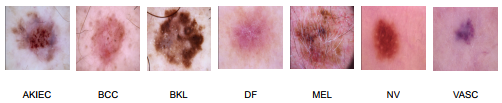
\includegraphics[width=1\linewidth]{Definitions/DataDistribution}
	\caption{\hl{Example} %MDPI: 1. Please cite the figure in the text and ensure the first citation of each figure appears in numerical order. 2. Please confirm if the vertical line is necessary, if not, please remove it.
 image of each~class.}
	\label{fig:data-sample}
\end{figure}

More than 50\% of lesions are confirmed through histopathology (HISTO); the~ground truth for the rest of the cases is either follow-up examination (FOLLOWUP), expert consensus (CONSENSUS), or~confirmation by in vivo confocal microscopy (CONFOCAL). On~the other hand, before~being used for training, the whole data are shuffled and then split into two parts. Here, $90$\% and $10$\% of the data is used for training and validating respectively. Images in this data set have the type of $RGB$ and shape of (450, 600). However, each backbone needs different input sizes of images as well as the range of pixel~value.

\subsubsection{Metadata}
The HAM10000 data set~\cite{10417} also contains the metadata of each patient including gender, age, and~the capturing position, as illustrated in Table~\ref{table:metadata sample}.
\begin{table}[H]\setlength{\tabcolsep}{11.7mm}

	\caption{\hl{Metadata} example in the data~set.}%MDPI: Please confirm if the vertical line is necessary, if not, please remove it.
	\label{table:metadata sample}
	\begin{tabular}{|c c c c |} 
	\noalign{\hrule height 1pt}

		\textbf{ID} & \textbf{Age} & \textbf{Gender} & \textbf{Local}\\ 
		\hline
		ISIC-00001 & 15 & Male & back\\
		\hline
		ISIC-00002 & 85 & Female & elbow\\
		\noalign{\hrule height 1pt}

	\end{tabular}
\end{table}
\unskip
\subsection{Methodology}
\unskip
\subsubsection{Overall~Architecture}
The whole architecture of the model is represented in the Figure~\ref{fig:main-model}. The~model takes two input including Image data and Metadata. The metadata branch, otherwise, is preprocessed before feeding into a dense layer; then, it concatenates with the output of the Soft-Attention~layer. 

\begin{figure}[H]
	%\centering
	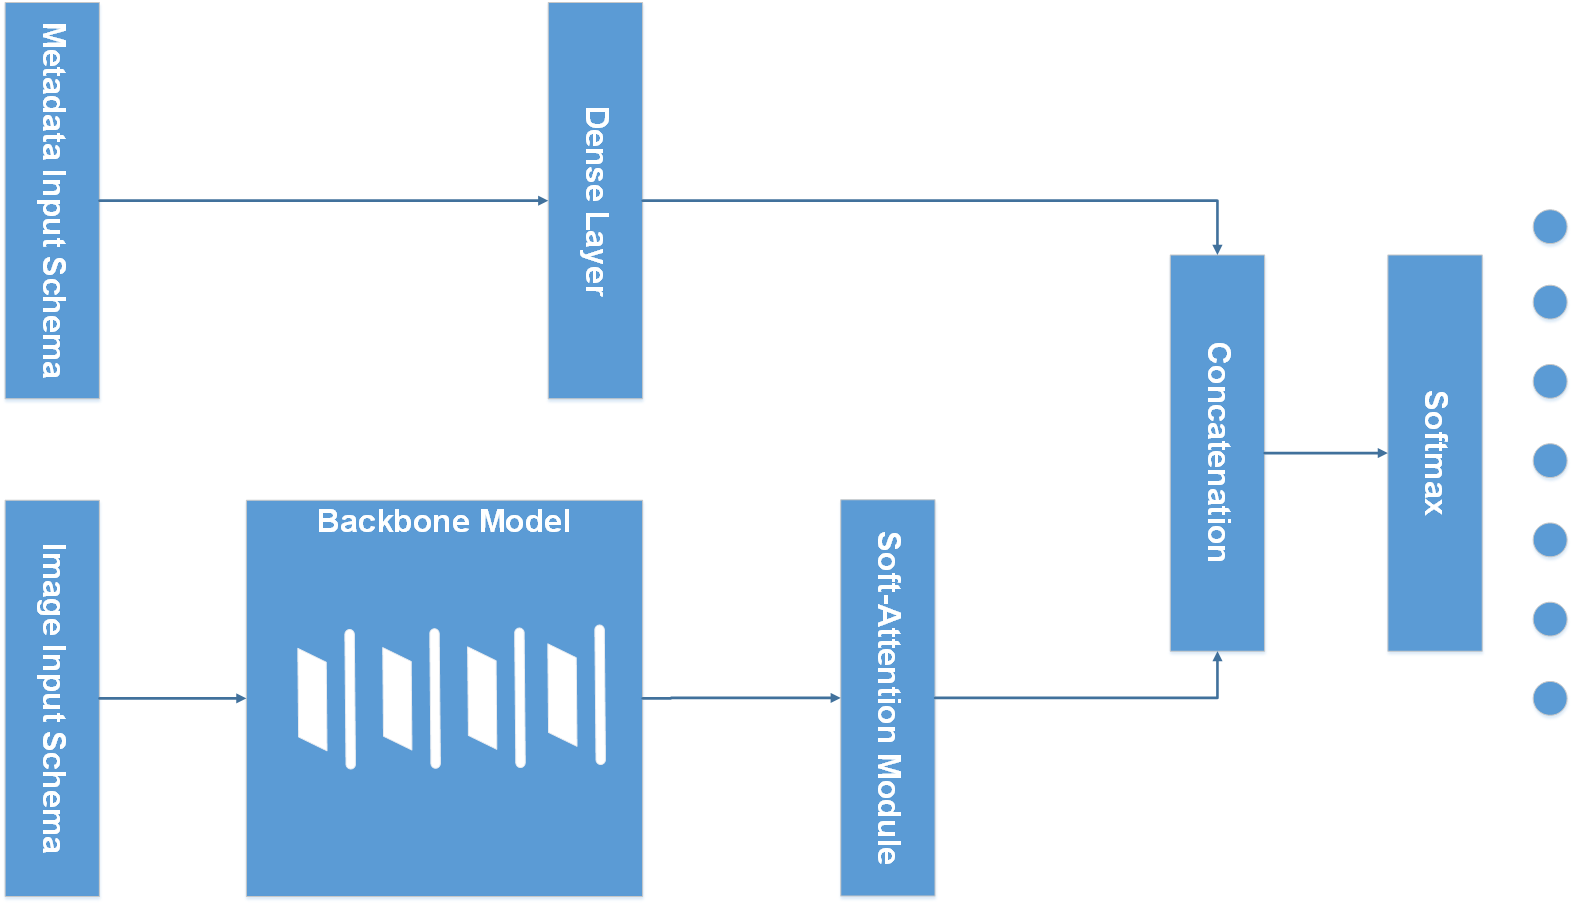
\includegraphics[width=0.8\linewidth]{Definitions/MainModel - Model Form}
	\caption{Overall Model~Architecture.}
	\label{fig:main-model}
\end{figure}

Figure~\ref{fig:model-structure} illustrates the overall structures of the combination of backbone models and Soft-Attention, which is used in this research. In~detail, the combination of DenseNet201 and Soft-Attention is formed by replacing the three last (DenseBlock, Global Average Pooling, and~the fully connected layer) with the Soft-Attention Module. Similarity, ResNet50 and ResNet152 also replaced the last three (Residual Block, Global Average Pooling, and~the fully connected layer) with the Soft-Attention module. InceptionResNetV2, on~the other hand, replaces the average pool and the last dropout with the Soft-Attention Module. The~last two, Normal Cell in NasNetLarge, is replaced with the Soft-Attention~module. 

\begin{figure}[H]
	%\centering
	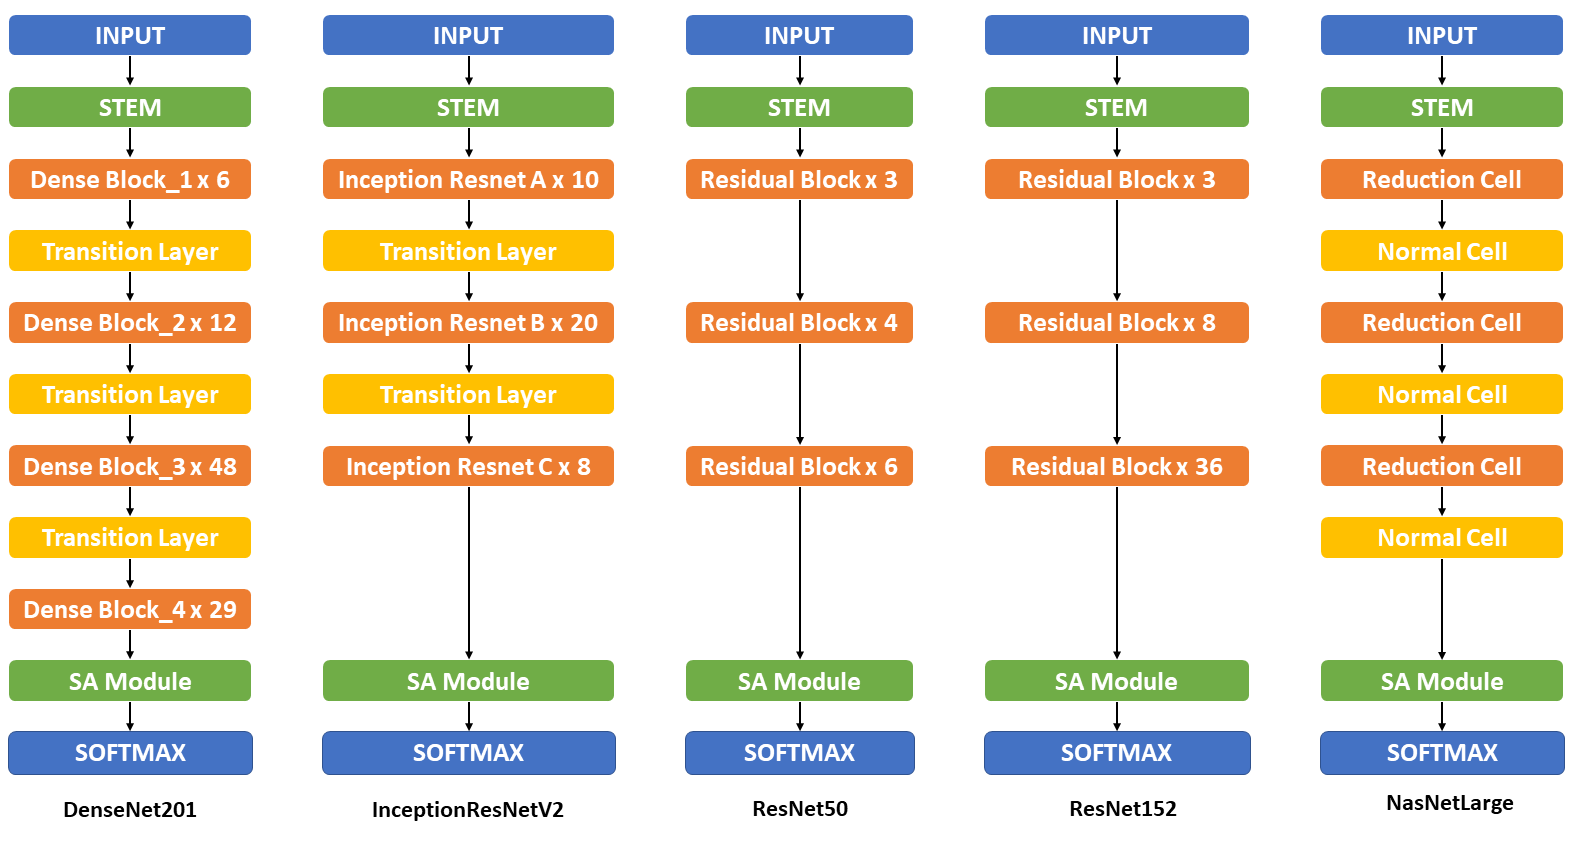
\includegraphics[width=0.8\linewidth]{Definitions/Model Structure}
	\caption{\hl{Overall Original} %MDPI: Please revise the "x" into a multiplication sign ("\times" U+00D7)
 Model Architecture. This figure show the overall structure of the backbone model (non mobile-based model) including DenseNet201, InceptionResNetV2, ResNet50, ResNet152, and~NasNetLarge. The~detailed structure and information can be found in Appendix \ref{app1} Table \ref{appendix-table:detailed structure model}.}
	\label{fig:model-structure}
\end{figure}

Figure~\ref{fig:mobile-model-structure}, on~the other hand, shows the detailed structure of the mobile-based mobile and its combination with Soft-Attention. All of the MobileNet versions combine with the Soft-Attention module by replacing the two last convolution layers 1 \hl{$\times$} %MDPI: We revised the "x" into a multiplication sign ("\times" U+00D7). Please confirm.
 1 with the Soft-Attention module. The~NasNetMobile, otherwise, combines with the Soft-Attention module by replacing the last normal~cell. 
\begin{figure}[H]
	%\centering
	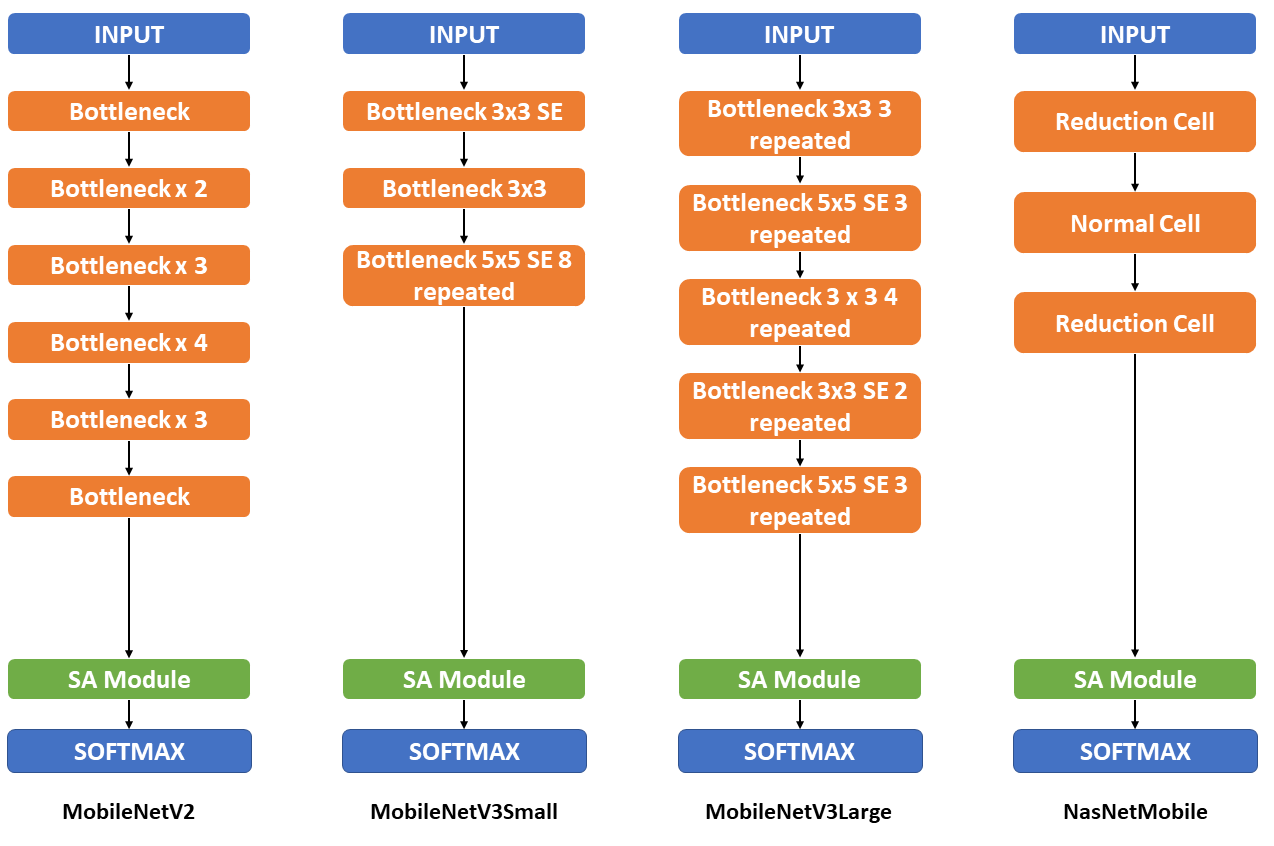
\includegraphics[width=0.8\linewidth]{Definitions/Mobile Model Structure}
	\caption{\hl{Overall mobile-based} %MDPI: Please revise the "x" into a multiplication sign ("\times" U+00D7)
 model architecture. This figure shows the overall structure of the mobile-based backbone model including MobileNetV2, MobileNetV3Small, MobileNetV3Large, and~NasNetMobile. The~detailed structure and information can be found in Appendix \ref{app2} Table  \ref{appendix-table:detailed mobile model structure}.}
	\label{fig:mobile-model-structure}
\end{figure}
\unskip

\subsubsection{Input~Schema}
In this research, the~image data are both augmented for all classes, the~number of images increases to 18,015 images, and it keeps the original form. Before~feeding into the backbone model, the~images are preprocessed by the input requirement of each model. DenseNet201~\cite{06993} requires the input pixels values to be scaled between $0$ and $1$ and each channel is normalized with respect to the ImageNet data set. In~Resnet50 and Resnet152~\cite{03385,05027}, the~images are converted from $RGB$ to $BGR$; then, each color channel is zero-centered with respect to the ImageNet data set without~scaling. InceptionResNetV2~\cite{11946}, on~the other hand, will scale input pixels between $-1$ and $1$. Similarly, three versions of MobileNet~\cite{04861,04381,02244}, NasNetMobile and NasNetLarge~\cite{07012} require the input pixel is in range of $-1$ and $1$. 

On the other hand, the~metadata are also used as another input. In~the research~\cite{03910}, they decide to keep the missing value and set its value to $0$. The~sex and anatomical site are categorical encoded. The~age, on~the other hand is numerical normalized. After~processing, the~metadata are fed into a two-layer neural network with 256 neurons each. Each layer contains batch normalization, a~ReLU~\cite{08375} activation, and~dropout with $p = 0.4$. The~network’s output is concatenated with the CNN’s feature vector after global average pooling. Especially, they use a simple data augmentation strategy to address the problem of missing values in metadata. During~training, they randomly encode each property as missing with a probability of $p = 0.1$. 

In this research, the~unknowns are kept as a type as discussed in Metadata section. Sex, anatomical site and age are also category encoded and numerical normalized, respectively. After~processing, the~metadata are then concatenated and fed into a dense layer of 4096~neurons. Finally, this dense layer is then concatenated with the output of Soft-Attention, which is then discussed in the Soft-Attention section. The~Input schema is described in \hl{Figure} %MDPI: We changed Table to Figure. Please confirm this revision.
 \ref{fig:input-schema}.

\begin{figure}[H]
%	\centering
	\includegraphics[width=1\linewidth]{"Definitions/Input Schema"}
	\caption{Input~Schema.}
	\label{fig:input-schema}
\end{figure}
\unskip

\subsubsection{Backbone~Model}
In this paper, the~backbone models used in this paper are DenseNet201~\cite{06993}, Inception~\cite{00567}, MobileNets~\cite{04861,04381,02244}, ResNet~\cite{03385,05027}, and~NasNet~\cite{07012}. The~combination of DenseNet201, InceptionResNetV2 and the Soft-Attention layer are both tested by the previous paper~\cite{03358} with a great performance. Otherwise, Resnet50 also well classifies but with much fewer parameters and less depth than based on its f1-score and precision stated. Therefore, in~this paper, the~performance of the Resnet152 and NasnetLarge models, which have more parameters and depth, is analyzed. On~the other hand, three versions of MobileNet and the NasnetMobile will also be analyzed, which has fewer parameters and~depth. 

\begin{table}[H]\setlength{\tabcolsep}{7.9mm}
\renewcommand{\arraystretch}{1.2}

	\caption{\hl{Size,} %MDPI: 1. Please cite the table in the text and ensure the first citation of each table appears in numerical order. 2. Please confirm if the vertical line is necessary, if not, please remove it.
 parameters, and depth of the backbone model used in this~paper.}
	\label{table:model-summary}
	\begin{tabular}{|l | c c c|} 
		\noalign{\hrule height 1pt}

		\textbf{Model} &\textbf{ Size (MB)} & \textbf{Parameters} & \textbf{Depth} \\ 
		\hline
		Resnet50 & 98 & 25.6 M & 107 \\ 
		\hline
		Resnet152 & 232 & 60.4 M & 311 \\ 
		\hline
		DenseNet201 & 80 & 20.2 M & 402 \\
		\hline
		InceptionResNetV2 & 215 & 55.9 M & 449 \\
		\hline
		MobileNet & 16 & 4.3 M & 55 \\ 
		\hline
		MobileNetV2 & 14 & 3.5 M & 105 \\ 
		\hline
		MobileNetV3Small & Unknown & 2.5 M & 88 \\ 
		\hline
		MobileNetV3Large & Unknown & 5.5 M & 118 \\
		\hline
		NasnetMobile & 23 & 5.3 M & 308 \\
		\hline
		NasnetLarge & 343 & 88.9 M & 533 \\ 
	\noalign{\hrule height 1pt}
	\end{tabular}
\end{table}
\unskip

\subsubsection{Soft-Attention~Module}
Soft-Attention has been used in various applications: image caption generation such as~\cite{03044} or handwriting verification~\cite{202017}. Soft-Attention can ignore irrelevant areas of the image by multiplying the corresponding feature maps with low weights. Soft-Attention is described in the below equation:
\[
f_{sa} = \gamma t\sum_{k=1}^{K}softmax(W_k * t)
\]
Figure~\ref{fig:soft-attention} shows the two main steps of applying Soft-Attention. Firstly, the~input tensor is put in grid-based feature extraction from the high-resolution image, where each grid cell is analyzed in the whole slide to generate a feature map~\cite{08513}. This feature map called $t \in R^{h \times w \times d}$ where $h, w, \text{and } d$ is the shape of tensor generated by a Convolution Neural Network (CNN) is then input to a 3D convolution layer whose weights are $W_k \in R^{h \times w \times d \times K}$. The~output of this convolution is normalized using the soft-max function to generate \hl{K} %MDPI: Please change the forward italics of the variables in the text and formulas to be consistent
 (a constant value) attention maps. These $K$ attention maps are aggregated to produce a weight function called $\alpha$. This $\alpha$ function is then multiplied with feature tensor $t$ and scaled by $\gamma$, which is a~learnable scalar. Finally, the~output of Soft-Attention function $f_{sa}$ is the concatenation of the beginning feature tensor $t$ and the scaled attention~maps. 

\begin{figure}[H]
	%\centering
	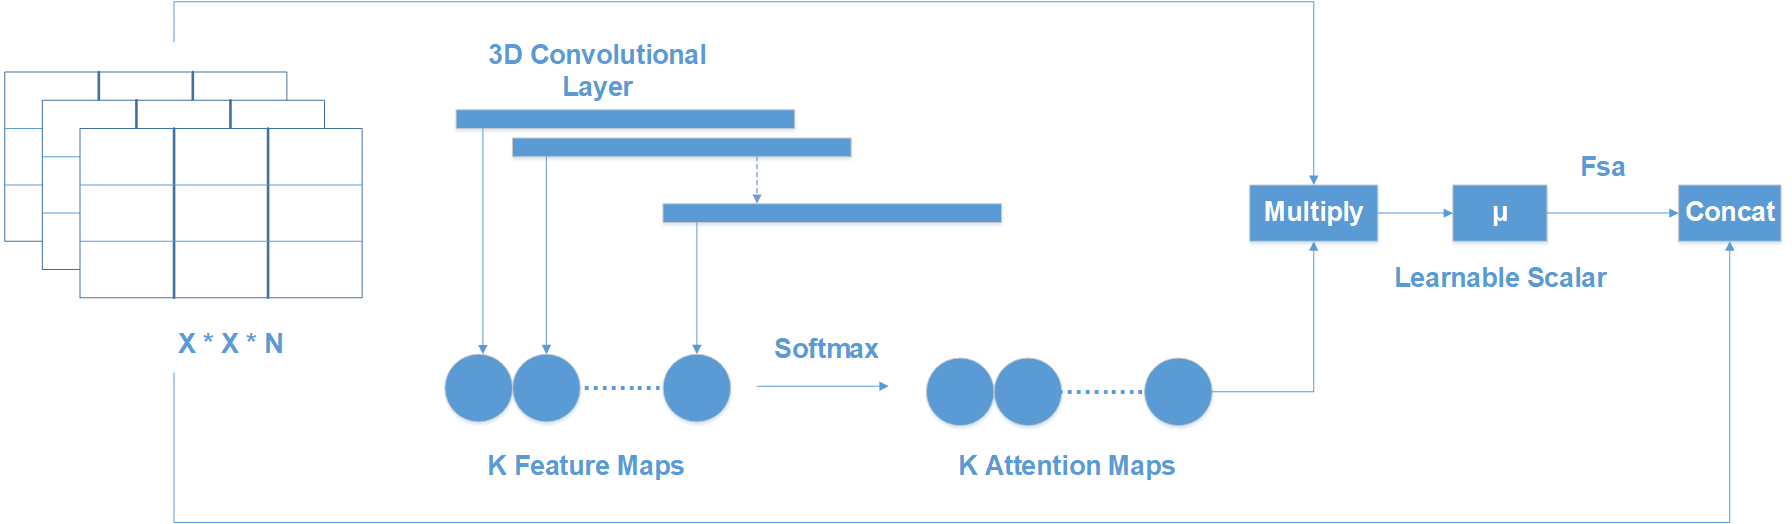
\includegraphics[width=1\linewidth]{Definitions/SoftAttention}
	\caption{\hl{Soft-Attention~Layer.} %MDPI: Please revise the "*" into a multiplication sign ("\times" U+00D7)
}
	\label{fig:soft-attention}
\end{figure}

In this research, the~Soft-Attention layer is applied in the same way in this research~\cite{03358}. The~Soft-Attention module is described in Figure~\ref{fig:soft-attention-block}.

\begin{figure}[H]
	%\centering
	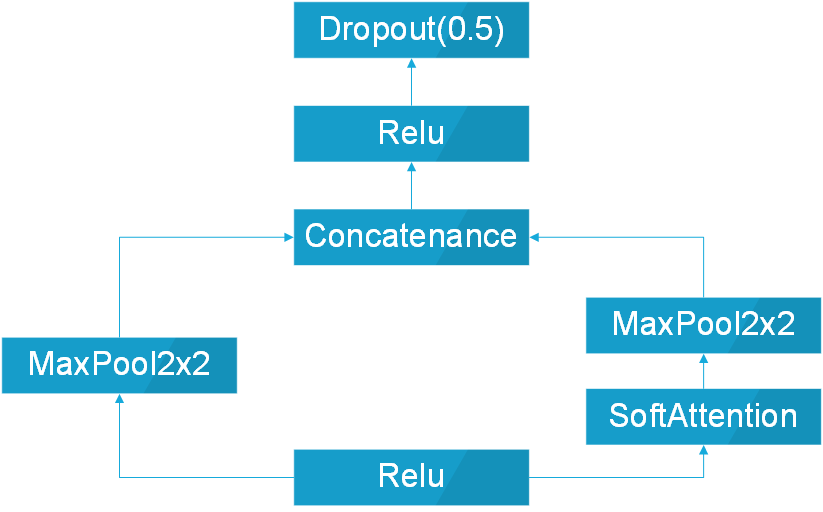
\includegraphics[width=0.5\linewidth]{Definitions/SoftAttentionBlock}
	\caption{\hl{Soft-Attention~Module.} %MDPI: Please revise the "x" into a multiplication sign ("\times" U+00D7)
}
	\label{fig:soft-attention-block}
\end{figure}

After feeding into the ReLU function layer, the~heat feature map is processed in two paths. The~first path is the two-dimensional Max Pooling. In~the second path, the~feature map, on~the other hand is fed into the Soft-Attention layer before the two-dimensional Max Pooling. After~all, these two paths are then concatenated and fed into a ReLU layer with~a dropout with the probability of $0.5$.


\subsubsection{Loss~Function}
The loss function used in this paper is categorical cross-entropy. Consider $X = [x_1, x_2, \dots, x_n]$ as the input feature $\theta = [\theta_1, \theta_2, \dots, \theta_n]$. Let $N$, and~$C$ be the number of training examples and number of classes, respectively. The~categorical cross-entropy loss is presented as:
\[L(\theta, x_n) = -\frac{1}{N}\sum_{c=1}^{C}\sum_{n=1}^{N}W_c\times y^c_n \times \log(\hat{y}^c_n)\]
where $\hat{y}^c_i$  is the output of the model, $y^c_i$ is the target that the model should return, and $W_c$ is the weight of class $c$. Since the data sets face the imbalanced problem, then class weight for the loss is applied. In~this research, both the original weight and a new weight formula are implemented. Originally, the~weight is calculated by taking the inverse of percentage that each class accounts for. The~new weight formula is described as follows:
\[W = N \odot D\]
\[D = \begin{bmatrix}
	\frac{1}{C \times  N_1} & \frac{1}{C \times  N_2} & \dots & \frac{1}{C \times  N_n}\\
\end{bmatrix} = \frac{1}{C} \odot \begin{bmatrix}
	\frac{1}{N_1} & \frac{1}{N_2} & \dots & \frac{1}{N_n}\\
\end{bmatrix}\]
where $N$ is the number of training samples, $C$ is the number of classes, $N_i$ is the number of samples in each class $i$. $D$ is the matrix that contains the inverse of $C \times N_i$. 

%%%%%%%%%%%%%%%%%%%%%%%%%%%%%%%%%%%%%%%%%%
\section{Results}
\unskip
\subsection{Experimental~Setup}
\unskip
\subsubsection{Training}
Before training, the~data set is split into two subsets for training (90\%) and validation (10\%). The test set otherwise is provided by the HAM10000 data set, and it contains 857 images. To~analyze the effect of augmented data on the model, before~the training, the image data are augmented to 53573 images by the following technique:




\begin{itemize}
\item[-]	Rotation range: rotate the image in a fixed~angle.
\item[-]		Width and height shift range: Shift the image horizontally and vertically, respectively.
\item[-]		Zoom range:  Zoom in or zoom out the image to create new~image. 
\item[-]		Horizontal and vertical flipping: Flipping the image horizontally and vertically to create new~image.
\end{itemize}




Otherwise, all of the models are trained with the Adam Optimizer~\cite{6980} with the learning rate of $0.001$, which is reduced by a factor of $0.2$ to a minimum learning rate of \hl{$0.1 \times 10^6$}%MDPI: We revised the "x" into a multiplication sign ("\times" U+00D7). Please confirm.
, and~the epsilon is set to $0.1$. The~initial epochs is set to 250~epochs, and the Early Stopping is also applied to stop the training, as the accuracy of the validation set does not increase after $25$ epochs. The~batch size is set to $32$.

\subsubsection{Tools}
TensorFlow and Keras are two of the most popular frameworks to build deep learning models. In~this research, Keras based on TensorFlow is used to build and clone the backbone model, which is pre-trained with the Image-Net data set. Otherwise, the~models are trained by NVIDIA RTX TitanV, and the data set is preprocessed with the CPU Intel I5 32 processors, RAM 32~GB. In~detail, the~GPU is set up with CUDA 11.6, cuDNN 8.3 and ChipSRT as the requirement of TensorFlow version~2.7.0.
\subsubsection{Evaluation~Metrics}

The model is evaluated by using the confusion matrix and related metrics. The \mbox{Figure~\ref{fig:confusion-matrix}} illustrates the presentation of a $2 \times 2$ confusion matrix used for class $2$. Consider a confusion matrix $A$ with $C$ number of classes. Let $A^i$ and $A^j$ be the set of $A$ rows and columns, respectively; therefore $A^i_k$ is the element at row i and column k.
\[
A = \begin{bmatrix}
	a_{11} & a_{12} & \dots & a_{1j} \\
	a_{21} & a_{22} & \dots & a_{2j} \\
	\vdots & \vdots	&  & \vdots\\
	a_{i1} & a_{i2} & \dots & a_{ij} 
\end{bmatrix}
\]

\vspace{-12pt}


\begin{figure}[H]
	\begin{minipage}{0.48\textwidth}
	%	\centering
		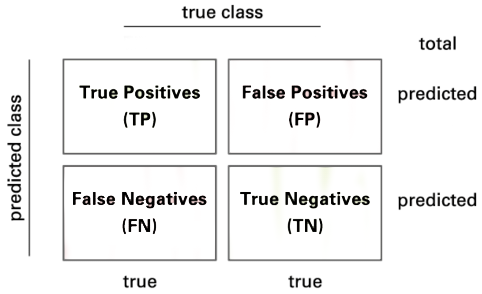
\includegraphics[width=1.1\linewidth]{Definitions/Confusion-matrix}
		\caption{Confusion~Matrix.}\label{fig:confusion-matrix}
	\end{minipage}
	
\end{figure}

\vspace{-12pt}

\begin{figure}[H]

	\begin{minipage}{0.48\textwidth}
		%\centering
		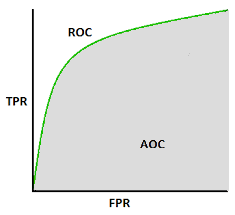
\includegraphics[width=.7\linewidth]{Definitions/AUC}
		\caption{\hl{Area Under} %MDPI: Please cite the figure in the text and ensure the first citation of each figure appears in numerical order.
 the~Curve.}\label{fig:AUC}
	\end{minipage}
\end{figure}



The True Positive (\hl{TP}%MDPI: Please change the forward italics of the variables in the text and formulas to be consistent
) of all classes in this case is the main diagonal of the matrix $A$. The~following methods are used to calculate the False Positives (\hl{FP}%MDPI: Please change the forward italics of the variables in the text and formulas to be consistent
), False Negatives (\hl{FN}%MDPI: Please change the forward italics of the variables in the text and formulas to be consistent
), and~True Negatives (\hl{TN}%MDPI: Please change the forward italics of the variables in the text and formulas to be consistent
) of all classes:
\[
FP = -TP + \sum_{k=1}^{i}A^i_k \hspace{1cm} FN = -TP + \sum_{k=1}^{j}A^j_k
\]
\[
TN_c = \sum_{i=1}^{C}\sum_{j=1}^{C}a_{ij} - \left[ \sum_{k=1}^{i}A^i_{i=c k} + \sum_{k=1}^{j}A^j_{j=c k} \right] + a_{i=c j=c} \implies TN = \begin{bmatrix}
	TN_1 & TN_2 & \dots & TN_c
\end{bmatrix}
\]
\hl{Then,} %MDPI: Please confirm should the no indentation be retained
 the~model is evaluated by the following metrics:
\[\text{Sensitivity(Sens)} = \frac{TP}{TP + FN} \hspace{1cm} \text{Specificity(Spec)} = \frac{TN}{TN + FP}\]
where Sensitivity and Specificity mathematically describe the accuracy of a test which reports the presence or absence of a condition. Individuals for which the condition is satisfied are considered ``positive'' and those for which it is not are considered ``negative''. Sensitivity or the True Positive rate refers to the probability of a positive test, which is conditioned on truly being positive while Specificity  or the True Negative rate refers to the probability of a negative test, which is conditioned on truly being negative.
\[\text{Precision} = \frac{TP}{TP + FP} \hspace{1cm} \text{F1 Score} = \frac{2 \times TP}{2 \times TP + FP + FN + TN}\]
\hl{Precision} %MDPI: Please confirm should the no indentation be retained
 or positive predictive value (PPV) is the probability of a positive test conditioned on both truly being positive or negative. F1-score, on~the other hand, refers the harmonic mean of precision and recall, which means the higher the f1-score is, the~higher both precision and recall are. The~expected value of precision, f1-score and recall score are also applied because of the multi-class problem.
\[\text{Accuracy} = \frac{TP + TN}{TP + FP + FN + TN} \hspace{1cm} \text{Balanced Accuracy} = \frac{\text{Sens} + \text{Spec}}{2}\]
\hl{The last} %MDPI: Please confirm should the no indentation be retained
 metric is the $AUC$ score standing for Area Under the Curve, which is the Receiver Operating Curve (ROC) that indicates the probability of TP versus the probability of~FP.  

\subsection{Discussion} 
\begin{comment}
	\begin{figure}[H]
		\centering
		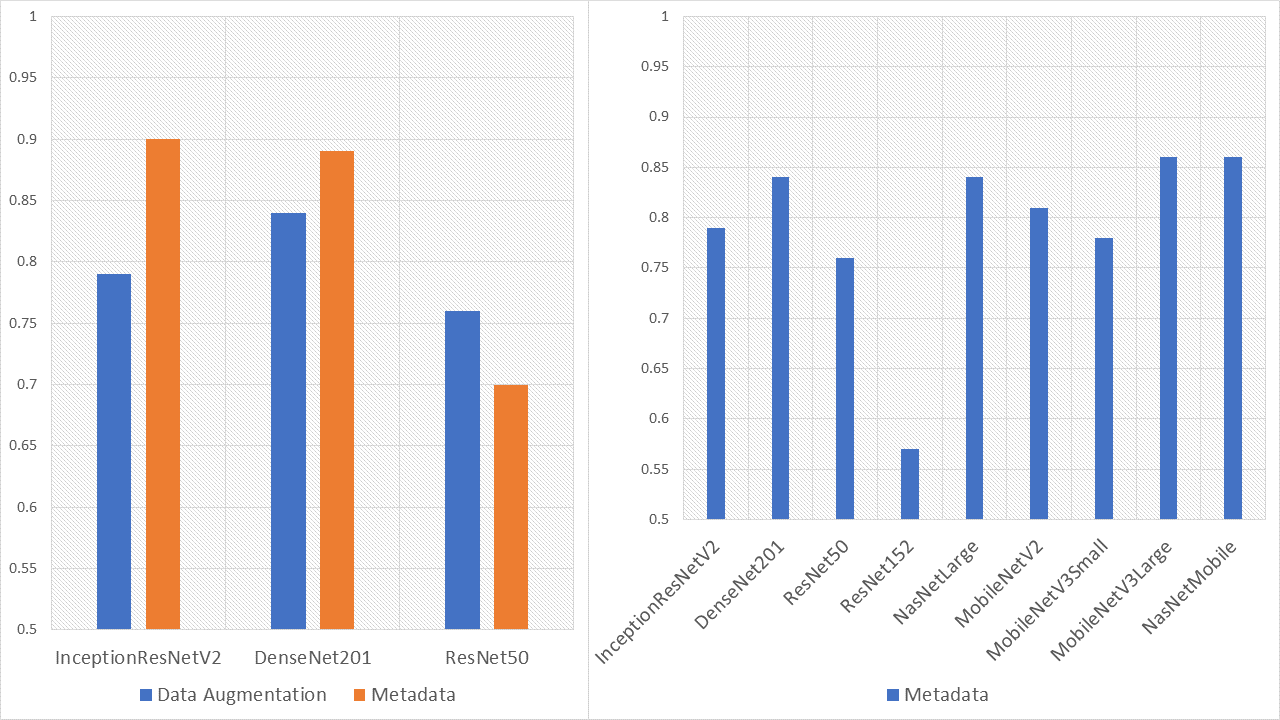
\includegraphics[width=1\linewidth]{Definitions/ACCALL}
		\caption{Accuracy of all models trained in this~research}
		\label{fig:accall}
	\end{figure}
\end{comment}

According to Table~\ref{table:overall-acc}, it is clear that the model trained with metadata has a higher accuracy than the model trained with augmented data only. While InceptionResNetV2 and DenseNet201 trained with augmented data have accuracy of $0.79$ and $0.84$, respectively, their training with metadata are $0.90$ and $0.89$, respectively. Furthermore, Resnet50 trained with metadata data has the accuracy that outperforms the Resnet50 trained with augmented data and is twice as high as Resnet152 trained with metadata. On~the other hand, mobile models including MobileNetV2, MobileNetV3Large, and~NasNetMobile, even though they have a much smaller number of parameters and depth than the other models, have quite good accuracy scores of $0.81$, $0.86$, and $0.86$, respectively. 

\begin{table}[H]\renewcommand{\arraystretch}{1.2}\setlength{\tabcolsep}{12.3mm}
	\caption{Accuracy of all models. ACC stands for accuracy. AD stands for augmented data; this indicates that the model is trained with augmented data. MD stands for metadata, which indicates that the model is trained with~metadata.}
	\label{table:overall-acc}
	\begin{tabular}{| l | c  c | }
	\noalign{\hrule height 1pt}

		\textbf{Model} & \textbf{ACC (AD)} & \textbf{ACC (MD)}\\ 
		\hline
		InceptionResNetV2 & 0.79 & \textbf{\hl{0.90} %MDPI: 1. Please confirm if the bold should be retained. 2. Please confirm if the vertical line is necessary, if not, please remove it.
}\\
		\hline
		DenseNet201 & 0.84 & \textbf{0.89}\\
		\hline
		ResNet50 & 0.76 & 0.70\\
		\hline
		ResNet152 & 0.81 & 0.57\\
		\hline
		NasNetLarge & - & 0.84\\
		\hline
		MobileNetV2 & - & 0.81\\
		\hline
		MobileNetV3Small & - & 0.78\\
		\hline
		MobileNetV3Large & 0.85 & \textbf{0.86}\\
		\hline
		NasNetMobile & 0.84 & \textbf{0.86}\\
		\noalign{\hrule height 1pt}

	\end{tabular}
\end{table}

Moreover, the~model trained with augmented data does not only have low accuracy but the f1-score and the recall score also are imbalanced according to Figures~\ref{fig:den f1}--\ref{fig:incep recall}. As~a result, the augmented data model does not classify well on all classes, as InceptionResNetV2 trained on augmented data has an f1-score on class df and the akiec is just above $0.3$ and $0.4$, separately, while InceptionResNetV2 trained on metadata and the new weight loss can classify well in a balanced way according to Figure~\ref{fig:incep f1}. However, only DenseNet201, InceptionResNetV2, and~NasNetLarge whose depth are equal to or larger than 400 have balanced f1-scores on class. The~others still face the imbalanced term. Since this data set is not balanced, therefore, using augmented data can make the model more  biased to the class which has a larger sample. Although using the metadata still leads to model bias, it does contribute to the improvement of  the performance of the~model.

\begin{figure}[H]
	\centering
	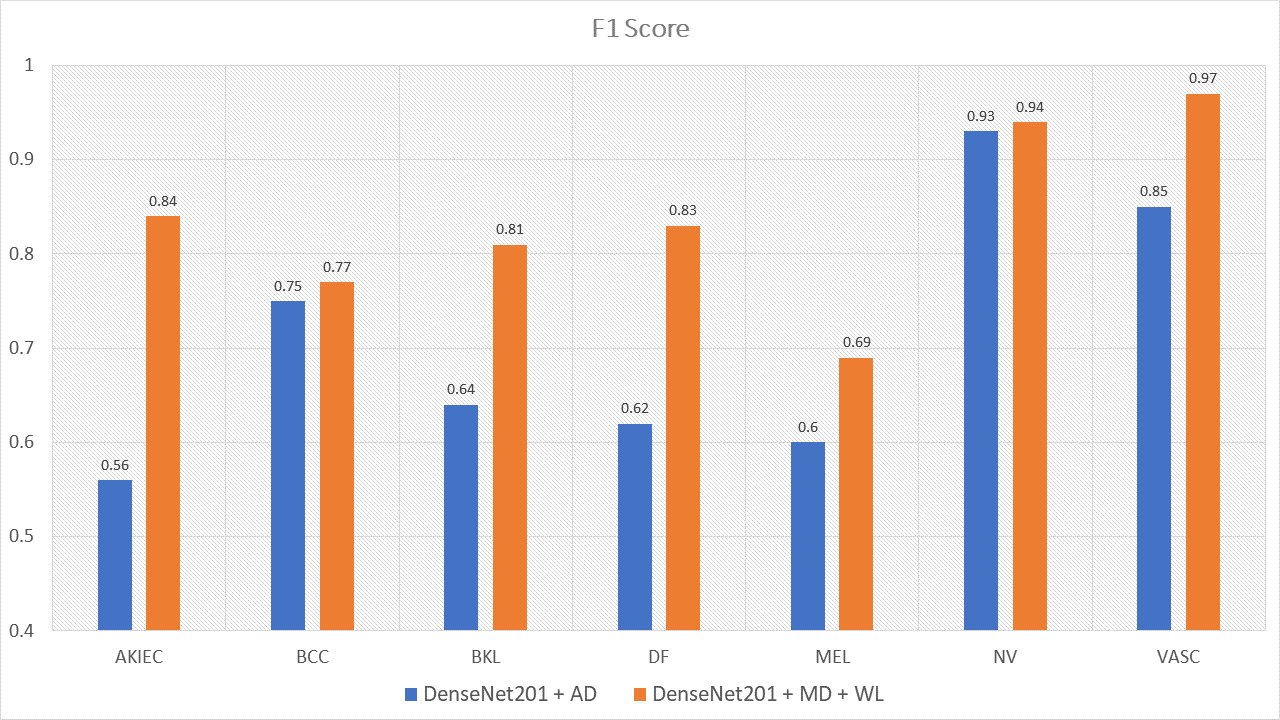
\includegraphics[width=1\linewidth]{Definitions/den f1}
	\caption{The comparison between f1-scores of DenseNet201 trained with augmented data and the one trained with metadata and weight~loss.}
	\label{fig:den f1}
\end{figure}
\unskip
\begin{figure}[H]
	\centering
	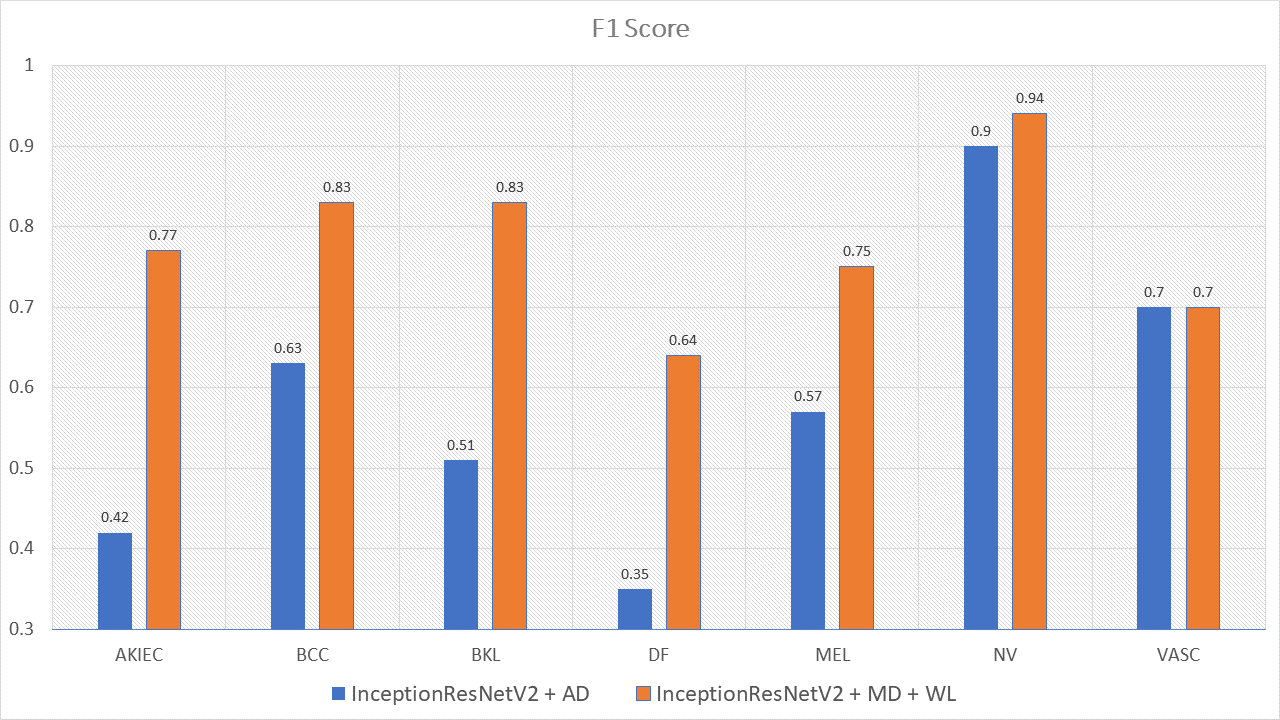
\includegraphics[width=1\linewidth]{Definitions/in f1}
	\caption{The comparison between f1-scores of InceptionResNetV2 trained with augmented data and the one trained with metadata and weight~loss.}
	\label{fig:incep f1}
\end{figure}

\textls[+25]{This problem is also true with the recall score according to Figures~\ref{fig:den recall} and \ref{fig:incep recall}.} DenseNet201 and InceptionResNetV2 trained with augmented data have expected recall values of $0.56$ and $0.69$, respectively, while the combination of DenseNet201, Metadata and the new weight loss function achieve the expected value of recall: $0.82$. Therefore, metadata do improve the model performance by reducing the amount of data needed for achieving higher results. On~the other hand, the~reason why the model becomes much more balanced is the weighted loss function. Weight loss function has the ability to solve the imbalanced class samples by adding a weight related to the number of samples in each class. DenseNet201 and InceptionResNetV2 trained with the new weighted loss function have recall in akiec of $0.85$ and $0.82$, respectively, as~opposed to their training in akiec without weighted loss function: $0.65$ and $0.37$. 

\begin{figure}[H]
	\centering
	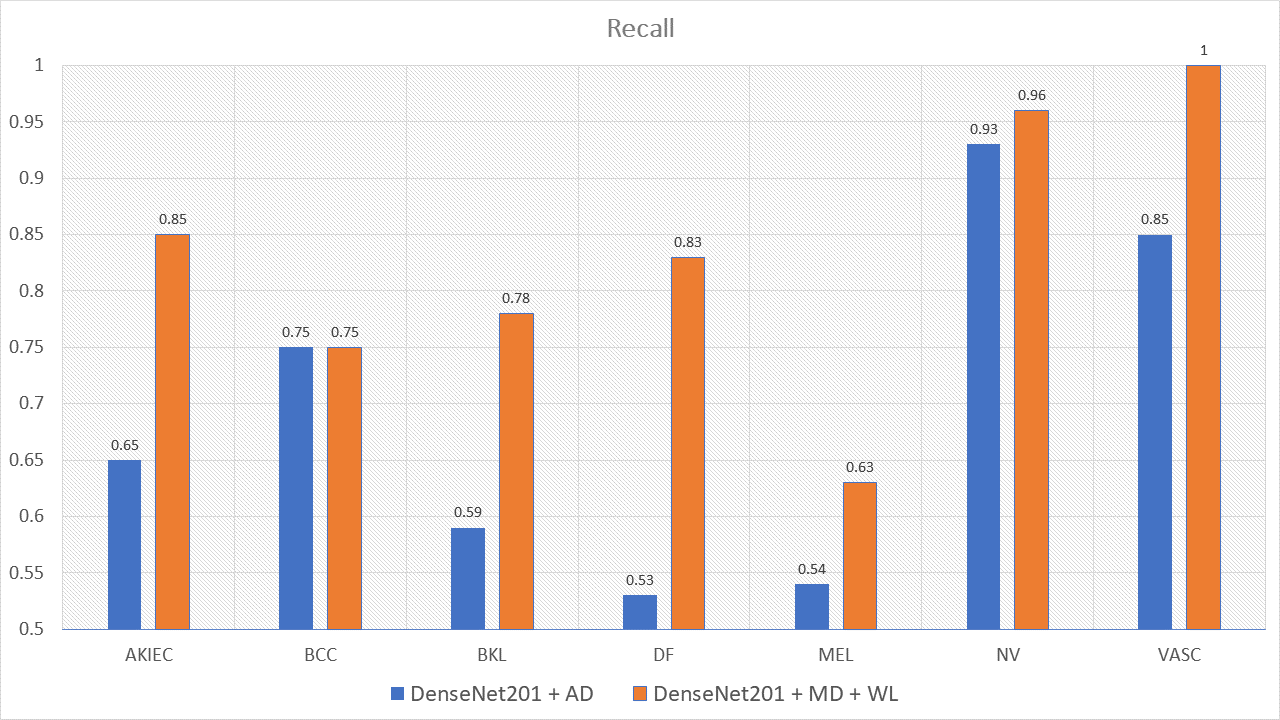
\includegraphics[width=1\linewidth]{Definitions/den re}
	\caption{The comparison between recal scores of DenseNet201 trained with augmented data and the one trained with metadata and weight~loss.}
	\label{fig:den recall}
\end{figure}
\unskip

\begin{figure}[H]
	\centering
	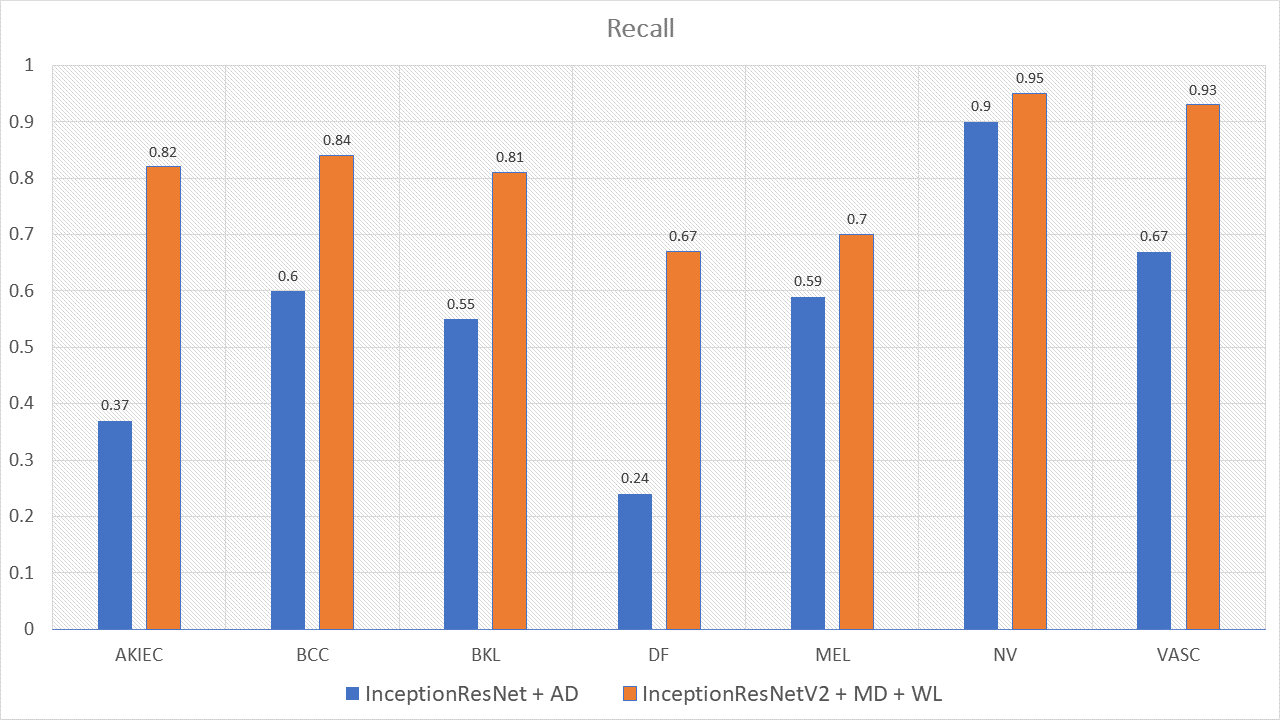
\includegraphics[width=1\linewidth]{Definitions/in re}
	\caption{The comparison between recall scores of InceptionResNetV2 trained with augmented data and the one trained with metadata and weight~loss.}
	\label{fig:incep recall}
\end{figure}

Another interesting point found during the experiment is that MobileNetV2, MobileNetV3 and NasNetMobile have a small number of parameters and depth, but they~have relatively good performance. MobileV3large, MobileV3Small, NasNetLarge and NasNetMobile outperform others on classifying class df with the recall scores of $0.92$, $1$, $0.92$, and $0.92$, separately, according to Table~\ref{appendix-table:mobile-performance}. It is transparent that MobileNetV3Large and NasNetMobile are the two best performance models. Nevertheless, MobileNetV3Large has fewer parameters and depth than~NasNetMobile.


Table~\ref{table:optimized-performance-mobile-model} shows that MobileNetV3Large, although~the number of parameters is much smaller than that of DenseNet201. InceptionResNetV2 achieves an accuracy near to the others. In~detail, MobileNetV3Large has 5.5 million parameters, which is four and ten times less than DenseNet201 and InceptionResNetV2, respectively. The~depth of MobileNetV3Large, on~the other hand, is four times less than DenseNet201, InceptionResNetV2, which is 118 hidden layers as opposed to the 402 and 449 values of DenseNet201 and InceptionResNetV2, separately. Although MobileNetV3Larege only achieves an accuracy of 0.86, the time needed for prediction is 10 and 30 times less than the other opponents. Since MobileNetV3Large needs a harder process of parameter hyper-tuning to achieve a better result, this is also the future target of this~research.




\begin{table}[H]\setlength{\tabcolsep}{1.6mm}\renewcommand{\arraystretch}{1.2}
	\caption{How the performance of MobileNetV3Large can be~optimized.}%MDPI: Please confirm if the vertical line is necessary, if not, please remove it.
	\label{table:optimized-performance-mobile-model}
	\begin{tabular}{| l | c | c | c |}
		\noalign{\hrule height 1pt}

		\textbf{Model} &\textbf{ MobileNetV3Large} & \textbf{DenseNet201 }& \textbf{InceptionResnetV2}\\
		\hline
		No. Parameters & \textbf{\hl{5.5 M} %MDPI: Please confirm if the bold should be retained.
} & 20.2 M & 55.9 M\\
		\hline
		Depth & \textbf{118} & 402 & 449\\
		\hline
		Accuracy & 0.86 & 0.89 & 0.90\\
		\hline
		Time Prediction(s/epochs) & \textbf{116} & 1000 & 3500 \\
	\noalign{\hrule height 1pt}

	\end{tabular}
\end{table}


Table~\ref{table:overall-auc} shows the AUC score of the three models---InceptionResNetV2, Densenet201, and~ResNet50---which are trained with only augmented data or metadata. It is transparent that InceptionResNetV2 and DenseNet201 have higher AUC-score trained with metadata: 0.974 and 0.971 as opposed to 0.972 and 0.93, respectively. ResNet50 trained with augmented data, on~the other hand, has a higher AUC-score: 0.95 as compared to 0.93 of ResNet50 trained with metadata. Overall, InceptionResNetV2 trained with metadata reaches the peak with an AUC score of 0.974. InceptionResNetV2 trained with metadata is also compared with the others to find out the best models trained. According to  \hl{\mbox{Figure~15},} %MDPI: There is no Figure 15 in the text, please revise.
InceptionResNetV2 still hit the peak AUC score of 0.974. In contrast, ResNet152 is the worst model with the AUC score of 0.87. Other models, on~the other hand, have the approximately the same AUC score. 

\begin{table}[H]\renewcommand{\arraystretch}{1.2}\setlength{\tabcolsep}{12.2mm}

	\caption{AUC (area under the curve) of all models. AD stands for augmented data; this indicates that the model is trained with augmented data. MD stands for metadata, which indicates that the model is trained with~metadata.}
	\label{table:overall-auc}
	\begin{tabular}{| l | c  c | }
	\noalign{\hrule height 1pt}

		\textbf{Model} & \textbf{AUC (AD)} & \textbf{AUC (MD)}\\ 
		\hline
		InceptionResNetV2 & 0.971 & \textbf{\hl{0.974} %MDPI: Please confirm if the bold should be retained.
}\\
		\hline
		DenseNet201 & 0.93 & \textbf{0.97}\\
		\hline
		ResNet50 & \textbf{0.95} & 0.93 \\
		\hline
		ResNet152 & - & 0.87\\
		\hline
		NasNetLarge & - & \textbf{0.96}\\
		\hline
		MobileNetV2 & - & \textbf{0.97}\\
		\hline
		MobileNetV3Small & - & \textbf{0.96}\\
		\hline
		MobileNetV3Large & - & \textbf{0.97}\\
		\hline
		NasNetMobile & - & \textbf{0.97}\\
		\noalign{\hrule height 1pt}
	\end{tabular}
\end{table}

%\clearpage 

In addition to the comparison between original weight loss calculated by the sample percentage of each class model and the new weight loss-based model, it is also conducted on the three best-performing models, including InceptionResNetV2, DenseNet201, and MobileNetV3. After~the experiment, it is found out that the new weight loss function does not only contribute to the model to overcome the data imbalance problem but it also makes the accuracy increase. The~performance of models is described in Table~\ref{table:loss-comparision}.

\begin{table}[H]\setlength{\tabcolsep}{2.75mm}\renewcommand{\arraystretch}{1.2}

	\caption{\hl{Loss}-based model accuracy~comparison.}%MDPI:  Please confirm if the vertical line is necessary, if not, please remove it.
	\label{table:loss-comparision}
	\begin{tabular}{| l | c | c | c |}
		\noalign{\hrule height 1pt}

		\textbf{Model} & \textbf{No Weight }& \textbf{Original Loss Accuracy} & \textbf{New Loss Accuracy}\\
		\hline
		InceptionResNetV2 & 0.74 & 0.79 & 0.90\\
		DenseNet201 & 0.81 & 0.84 & 0.89\\
		MobileNetV3 & 0.79 & 0.80 & 0.86\\
			\noalign{\hrule height 1pt}
	\end{tabular}
\end{table} 

After reviewing, InceptionResNetV2 is found to be the best model trained. Futhermore, InceptionResNetV2 is compared with the other state of the art researched models. According to Table~\ref{table:comparative-analysis}, there are six researchers that use the same data set: HAM10000, but they have different approaches. These models used in that research are also SOTA models sorted in ascending order. The~table shows that the accuracy of the combination of InceptionResNetV2 with Soft-Attention, metadata and weight loss in this research is less than that of InceptionResNetV2 with Soft-Attention and augmented data: 0.90 compared to 0.93, respectively. However, since Soumyyak et al. use data augmentation for all classes of an imbalanced data set, the~f1-score and recall score are much lower. This is because the model in that research can only classify well on NV and VASC classes, which have the highest number of samples. On~the other hand, InceptionResNetV2 in this research also outperforms the other models according to five indicators: accuracy, precision, f1-score, recall score, and~AUC score. 
\FloatBarrier
\begin{table}[H]\renewcommand{\arraystretch}{1.2}\setlength{\tabcolsep}{1.6mm}
	\caption{Comparative~Analysis.}%MDPI:  Please confirm if the vertical line is necessary, if not, please remove it.
	\label{table:comparative-analysis}
	\begin{tabular}{| l| c | c | c | c | c |}
		\noalign{\hrule height 1pt}

		\textbf{Model} & \textbf{Accuracy} & \textbf{Precision} & \textbf{F1-Score} & \textbf{Recall} & \textbf{Auc-Score}\\
		\hline
		Our Proposed & 0.9	& 0.86 &\textbf{\hl{0.86} %MDPI: Please confirm if the bold should be retained.
} & \textbf{0.81} & 0.974\\
		\hline
		InceptionResNetV2~\cite{03358} & 0.93 & 0.89 & 0.75 & 0.71 & 0.97\\
		\hline~\cite{03798} & - & 0.88 & 0.77 & 0.74 & - \\
		\hline~\cite{09418} & 0.88 & - & - & - & - \\
		\hline~\cite{01284} & 0.86 & - & - & - & - \\
		\hline
		GradCam and Kernel SHAP~\cite{06612} & 0.88 & - & - & - & - \\
		\hline
		Student and Teacher~\cite{03225} & 0.85 & 0.76 & 0.76 & - & - \\
			\noalign{\hrule height 1pt}
	\end{tabular}
\end{table} 

However, there is still some drawbacks of the model: InceptionResNetV2 cannot well classify the melanoma and the nevus. According to Figure~\ref{fig:nevusVSmela}, the model sometimes classifies the black nevus as the melanoma because of the same color between them. However, this problem is not true for the hard black or big melanoma or the red black nevus. Some future approaches that can be proposed would be to change the type of color to the other to fix the same color~problem.

\begin{figure}[H]
	%\centering
	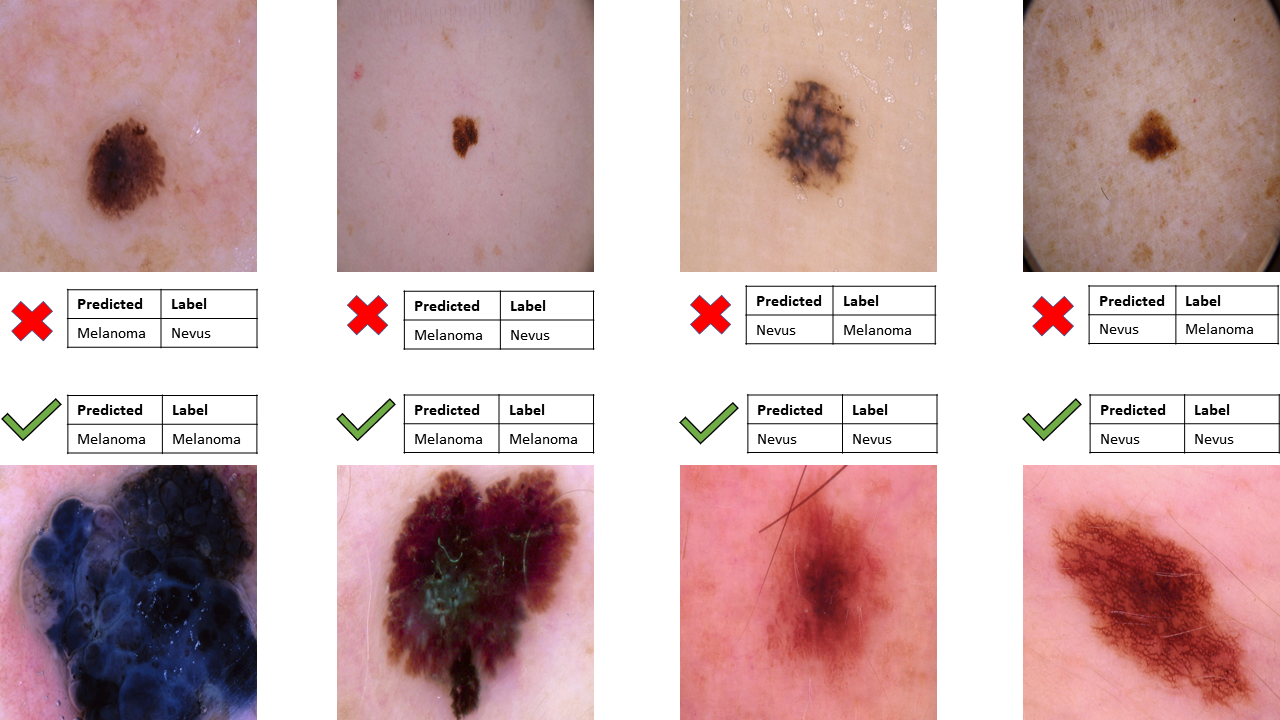
\includegraphics[width=0.9\linewidth]{Definitions/img_class_nevus_mela}
	\caption{Model ability to classify melanoma and~nevus.}
	\label{fig:nevusVSmela}
\end{figure}
\unskip

\section{Conclusions}
In this research, our proposal is to construct a model as a combination of backbone models and Soft-Attention. Moreover, the~model takes two inputs, including image data and metadata. A~new weight loss function is applied to figure out the data imbalance problem. Finally, the~combination of InceptionResNetV2, Soft-Attention, and~metadata is the best model. Although~the accuracy and the precision of the model are not the highest, the~f1-score, recall, and~AUC score are the highest and the most balanced indicators. Therefore, InceptionResnetV2 can classify well in all classes including low-samples classes. Otherwise, during~the experiment, the~combination of MobileNetV3, Soft-Attention, and~metadata achieves an accuracy that is nearly the same as InceptionResNetV2, although~with fewer  parameters and depth. Therefore, the infer time is much less than that of InceptionResNetV2. This result opens the door to constructing a great performance model that can be applied to mobile and IoT devices.  
\vspace{6pt} 

%%%%%%%%%%%%%%%%%%%%%%%%%%%%%%%%%%%%%%%%%%
%% optional
%\supplementary{The following supporting information can be downloaded at:  \linksupplementary{s1}, Figure S1: title; Table S1: title; Video S1: title.}

% Only for the journal Methods and Protocols:
% If you wish to submit a video article, please do so with any other supplementary material.
% \supplementary{The following supporting information can be downloaded at: \linksupplementary{s1}, Figure S1: title; Table S1: title; Video S1: title. A supporting video article is available at doi: link.}

%%%%%%%%%%%%%%%%%%%%%%%%%%%%%%%%%%%%%%%%%%
\authorcontributions{Conceptualization, V.D.N. and H.K.D.; methodology, V.D.N. and H.K.D.; software, K.D.; validation, V.D.N., N.D.B. and H.K.D.; formal analysis, V.D.N. and H.K.D.; investigation, V.D.N., N.D.B. and H.K.D.; resources, V.D.N.; data curation, H.K.D.; writing---original draft preparation, H.K.D.; writing---review and editing, V.D.N. and N.D.B.; visualization, H.K.D.; supervision, V.D.N. and N.D.B.; project administration, V.D.N. All authors have read and agreed to the published version of the~manuscript.}

\funding{This research received no external~funding.}

\institutionalreview{Not applicable.}

\informedconsent{Not applicable.}

\dataavailability{\textls[-15]{The code and the data analysis report can be found here:} \url{https://github.com/KhoiDOO/Skin-Disease-Detection-HAM100000.git}  (\hl{accessed on}%MDPI: Please add the access date (Format: Date Month Year) that earlier than Received date. e.g., (accessed on 29 August 2022).
).} 



\conflictsofinterest{The authors declare no conflict of~interest.} 

%%%%%%%%%%%%%%%%%%%%%%%%%%%%%%%%%%%%%%%%%%
%% Optional
%\sampleavailability{}

%% Only for journal Encyclopedia
%\entrylink{The Link to this entry published on the encyclopedia platform.}


\abbreviations{Abbreviations}{
The following abbreviations are used in this manuscript:\\

\noindent 
\begin{tabular}{@{}ll}
CAD & Computer-aided diagnosis\\
AI & Artificial intelligence\\
AKIEC~~~~~~~~~~~~~ & Actinic keratoses and intraepithelial carcinoma or Bowen's disease\\
BCC & Basal Cell Carcinoma\\
BKL & Benign Keratosis-like Lesions\\
\end{tabular}



\noindent 
\begin{tabular}{@{}ll}


DF & Dermatofibroma\\
MEL & Melanoma\\
NV & Melanocytic Nevi\\
VASC & Vascular Lesions\\
HISTO & Histopathology\\
FOLLOWUP & Follow-up examination\\
CONSENSUS & Expert Consensus\\
CONFOCAL & Confocal Microscopy\\
RGB & Red Green Blue\\
BGR & Blue Green Red\\
TP & True Positives\\
FN & False Negatives\\
TN & True Negatives\\
FP & False Positives\\
Sens & Sensitivity\\
Spec & Specificity\\
AUC & Area Under the Curve\\
ROC & Receiver Operating Curve\\
\end{tabular}
}

%%%%%%%%%%%%%%%%%%%%%%%%%%%%%%%%%%%%%%%%%%
%% Optional

%\startlandscape





\appendixtitles{yes} % Leave argument "no" if all appendix headings stay EMPTY (then no dot is printed after "Appendix A"). If the appendix sections contain a heading then change the argument to "yes".
\appendixstart
\appendix
\section[\appendixname~\thesection]{Detailed Model Structure}\label{app1}


\vspace{-6pt}

\begin{table}[H]\renewcommand{\arraystretch}{1.2}
	\caption{\hl{Detailed structure} %MDPI: 1. We revised the "x" into a multiplication sign ("\times" U+00D7). Please confirm. 2. Please confirm if the vertical line is necessary, if not, please remove it.
 of models except for mobile models. SA stands for Soft-Attention, SA Module denotes whether that model uses the Soft-Attention module. GAP stands for Global Average Pooling. FC stands for Fully Connected~Layer.\label{appendix-table:detailed structure model}}
    \tablesize{\scriptsize}	
	\begin{adjustwidth}{-\extralength}{0cm}
	

		%\newcolumntype{C}{>{\centering\arraybackslash}X}
%{\fontsize{7}{7}\selectfont
%\tablesize{\fontsize{7}{7}\selectfont}
%
%


\setlength{\cellWidtha}{\fulllength/10-2\tabcolsep-0in}
\setlength{\cellWidthb}{\fulllength/10-2\tabcolsep-0in}
\setlength{\cellWidthc}{\fulllength/10-2\tabcolsep-0in}
\setlength{\cellWidthd}{\fulllength/10-2\tabcolsep-0in}
\setlength{\cellWidthe}{\fulllength/10-2\tabcolsep-0in}
\setlength{\cellWidthf}{\fulllength/10-2\tabcolsep-0.01in}
\setlength{\cellWidthg}{\fulllength/10-2\tabcolsep-0.01in}
\setlength{\cellWidthh}{\fulllength/10-2\tabcolsep-0.01in}
\setlength{\cellWidthi}{\fulllength/10-2\tabcolsep-0.01in}
\setlength{\cellWidthj}{\fulllength/10-2\tabcolsep-0.01in}
\scalebox{1}[1]{\begin{tabularx}{\fulllength}{|>{\PreserveBackslash\raggedright}m{\cellWidtha}|>{\PreserveBackslash\raggedright}m{\cellWidthb}|>{\PreserveBackslash\raggedright}m{\cellWidthc}|>{\PreserveBackslash\raggedright}m{\cellWidthd}|>{\PreserveBackslash\raggedright}m{\cellWidthe}|>{\PreserveBackslash\raggedright}m{\cellWidthf}|>{\PreserveBackslash\raggedright}m{\cellWidthg}|>{\PreserveBackslash\raggedright}m{\cellWidthh}|>{\PreserveBackslash\raggedright}m{\cellWidthi}|>{\PreserveBackslash\raggedright}m{\cellWidthj}|}



	%\begin{tabularx}{\fulllength}{l|l|l|l|l|l|l|l|l|l}
			\noalign{\hrule height 1pt}

			\textbf{DenseNet-201} & \textbf{DenseNet-201 + SA} & \textbf{Inception-ResNetV2} & \textbf{Inception-ResNetV2 + SA} & \textbf{ResNet-50} & \textbf{ResNet-50 + SA} & \textbf{ResNet-152} & \textbf{ResNet-152 + SA} & \textbf{NasNet-Large} & \textbf{NasNet-Large + SA}\\
			\hline
			Conv2D \mbox{\mbox{7 $\times$ 7}} & Conv2D \mbox{7 $\times$ 7} & STEM& STEM& Conv2D \mbox{7 $\times$ 7}& Conv2D \mbox{7 $\times$ 7}& Conv2D \mbox{7 $\times$ 7}& Conv2D \mbox{7 $\times$ 7}& Conv2D \mbox{3 $\times$ 3}& Conv2D \mbox{3 $\times$ 3}\\ \hline
			Pooling \mbox{3 $\times$ 3} & Pooling \mbox{3 $\times$ 3} & & & Pooling \mbox{3 $\times$ 3}& Pooling  \mbox{3 $\times$ 3}& Pooling  \mbox{3 $\times$ 3}& Pooling  \mbox{3 $\times$ 3}& Pooling& Pooling\\ \hline		
			DenseBlock $\times$ 6 & DenseBlock $\times$ 6 & Inception ResNet A $\times$ 10& Inception ResNet A $\times$ 10& Residual Block $\times$ 3& Residual Block $\times$ 3& Residual Block $\times$ 3& Residual Block $\times$ 3& Reduction Cell $\times$ 2& Reduction Cell $\times$ 2\\  \hline
			Conv2D \mbox{1 $\times$ 1} & Conv2D \mbox{1 $\times$ 1} & Reduction A & Reduction A & & & & & Normal Cell $\times$ N& Normal Cell $\times$ N\\	\hline			
			Average pool \mbox{2 $\times$ 2} & Average pool \mbox{2 $\times$ 2} & & & & & & & & \\ \hline			
			DenseBlock $\times$ 12 & DenseBlock $\times$ 12 & Inception ResNet B $\times$ 20& Inception ResNet B $\times$ 20& Residual Block $\times$ 4& Residual Block $\times$ 4& Residual Block $\times$ 8& Residual Block $\times$ 8& Reduction Cell& Reduction Cell\\ \hline
			Conv2D \mbox{1 $\times$ 1} & Conv2D \mbox{1 $\times$ 1} & Reduction B & Reduction B & & & & & Normal Cell $\times$ N& Normal Cell $\times$ N\\			\hline
			Average pool \mbox{2 $\times$ 2} & Average pool \mbox{2 $\times$ 2} & & & & & & & & \\ \hline
			DenseBlock $\times$ 48 & DenseBlock $\times$ 12 & Inception ResNet C $\times$ 5& Inception ResNet C $\times$ 5& Residual Block $\times$ 6& Residual Block $\times$ 6& Residual Block $\times$ 36& Residual Block $\times$ 36& Reduction Cell& Reduction Cell\\ \hline
			Conv2D \mbox{1 $\times$ 1} & Conv2D \mbox{1 $\times$ 1} & & & & & & & Normal Cell $\times$ N& Normal Cell $\times$ N$-$2\\			\hline
			Average pool \mbox{2 $\times$ 2} & Average pool \mbox{2 $\times$ 2} & & & & & & & & \\ \hline
			DenseBlock $\times$ 29 & DenseBlock $\times$ 29 & & & Residual Block $\times$ 3& & Residual Block $\times$ 3& & & \\ \hline
			DenseBlock $\times$ 3 & \textbf{\hl{SA Module} %MDPI: Please confirm if the bold should be retained.
} & & \textbf{SA Module}& & \textbf{SA Module}& & \textbf{SA Module}& & \textbf{SA Module}\\	\hline
			GAP \mbox{7 $\times$ 7} & & Average pool& & GAP \mbox{7 $\times$ 7}& & GAP \mbox{7 $\times$ 7}& & & \\			\hline
			FC 1000D & & Dropout (0.8)& & FC 1000D& & FC 1000D& & & \\ \hline
			SoftMax & SoftMax & SoftMax& SoftMax& SoftMax& SoftMax& SoftMax& SoftMax& SoftMax& SoftMax\\ 			
			\noalign{\hrule height 1pt}
		\end{tabularx}
		}
		
	\end{adjustwidth}
\end{table}




%\finishlandscape



	
\section[\appendixname~\thesection]{Detailed Mobile-Based Model Structure}\label{app2}


\vspace{-6pt}

\begin{table}[H]\renewcommand{\arraystretch}{1.2}

	\caption{\hl{Detailed} structure of mobile-based models. SA stands for Soft-Attention, SA Module denotes whether that model uses the Soft-Attention module. SE stands for Squeeze-And-Excite, and it shows whether that block has~Squeeze-And-Excite. \label{appendix-table:detailed mobile model structure}}%MDPI: Please confirm if the vertical line is necessary, if not, please remove it.

    \tablesize{\footnotesize}	
	\begin{adjustwidth}{-\extralength}{0cm}
		%\newcolumntype{C}{>{\centering\arraybackslash}X}
		
		
		\setlength{\cellWidtha}{\fulllength/8-2\tabcolsep-0in}
\setlength{\cellWidthb}{\fulllength/8-2\tabcolsep-0in}
\setlength{\cellWidthc}{\fulllength/8-2\tabcolsep-0in}
\setlength{\cellWidthd}{\fulllength/8-2\tabcolsep-0in}
\setlength{\cellWidthe}{\fulllength/8-2\tabcolsep-0.01in}
\setlength{\cellWidthf}{\fulllength/8-2\tabcolsep-0.01in}
\setlength{\cellWidthg}{\fulllength/8-2\tabcolsep-0.01in}
\setlength{\cellWidthh}{\fulllength/8-2\tabcolsep-0.01in}
\scalebox{1}[1]{\begin{tabularx}{\fulllength}{|>{\PreserveBackslash\raggedright}m{\cellWidtha}|>{\PreserveBackslash\raggedright}m{\cellWidthb}|>{\PreserveBackslash\raggedright}m{\cellWidthc}|>{\PreserveBackslash\raggedright}m{\cellWidthd}|>{\PreserveBackslash\raggedright}m{\cellWidthe}|>{\PreserveBackslash\raggedright}m{\cellWidthf}|>{\PreserveBackslash\raggedright}m{\cellWidthg}|>{\PreserveBackslash\raggedright}m{\cellWidthh}|}



	%	\begin{tabularx}{\fulllength}{l|l|l|l|l|l|l|l|l}
			\noalign{\hrule height 1pt}
			\textbf{MobileNetV2} & \textbf{MobileNetV2 + SA} & \textbf{MobileNetV3 Small} & \textbf{MobileNetV3 Small + SA} & \textbf{MobileNetV3 Large} & \textbf{MobileNetV3 Large + SA} & \textbf{NasNet Mobile} & \textbf{NasNetMobile + SA}\\
			\hline
			Conv2D & Conv2D& Conv2D \mbox{3 $\times$ 3}& Conv2D \mbox{3 $\times$ 3}& Conv2D \mbox{3 $\times$ 3}& Conv2D \mbox{3 $\times$ 3} & Normal Cell & Normal Cell\\	\hline		
			bottleneck & bottleneck & bottleneck \mbox{3 $\times$ 3} SE& bottleneck \mbox{3 $\times$ 3} SE& bottleneck \mbox{3 $\times$ 3} 3 repeated& bottleneck \mbox{3 $\times$ 3} 3 repeated& Reduction Cell& Reduction Cell\\ \hline					
			bottleneck 2 repeated& bottleneck 2 repeated& bottleneck \mbox{3 $\times$ 3}& bottleneck \mbox{3 $\times$ 3}& bottleneck \mbox{5 $\times$ 5} SE 3 repeated& bottleneck \mbox{5 $\times$ 5} SE 3 repeated & Normal Cell & Normal Cell\\ \hline	
			bottleneck 3 repeated& bottleneck 3 repeated& bottleneck \mbox{5 $\times$ 5} SE 8 repeated& bottleneck \mbox{5 $\times$ 5} SE 8 repeated& bottleneck \mbox{3 $\times$ 3} 4 repeated& bottleneck \mbox{3 $\times$ 3} 4 repeated& Reduction Cell & Reduction Cell\\ \hline	
			bottleneck 4 repeated& bottleneck 4 repeated& & & bottleneck \mbox{3 $\times$ 3} SE 2 repeated& bottleneck \mbox{3 $\times$ 3} SE 2 repeated & Normal Cell&\\ \hline	
			bottleneck 3 repeated& bottleneck 3 repeated& & & bottleneck \mbox{5 $\times$ 5} SE 3 repeated& bottleneck \mbox{5 $\times$ 5} SE 3 repeated&& \\ \hline	
			bottleneck 3 repeated& bottleneck & & & & && \\ \hline	
			bottleneck & & & & & &&~ \\ \hline
			Conv2D \mbox{1 $\times$ 1} & & Conv2D \mbox{1 $\times$ 1} SE & Conv2D \mbox{1 $\times$ 1} SE& Conv2D \mbox{1 $\times$ 1}& Conv2D \mbox{1 $\times$ 1} & & \\ \hline
			AP \mbox{7 $\times$ 7} & & Pool \mbox{7 $\times$ 7}& Pool \mbox{7 $\times$ 7}& Pool \mbox{7 $\times$ 7}& Pool \mbox{7 $\times$ 7}& &~\\ \hline
			Conv2D \mbox{1 $\times$ 1} & \textbf{SA Module}& Conv2D \mbox{1 $\times$ 1} 2 repeated& \textbf{SA Module}& Conv2D \mbox{1 $\times$ 1} 2 repeated& \textbf{SA Module}& &\textbf{SA Module}\\ \hline
			Softmax & Softmax& Softmax& Softmax& Softmax& Softmax& Softmax & Softmax\\ 
			\noalign{\hrule height 1pt}
		\end{tabularx}}
	\end{adjustwidth}
\end{table}

%%%%%%%%%%%%%%%%%%%%%%%%%%%%%%%%%%%%%%%%%%



\section[\appendixname~\thesection]{Detailed Model Performance}
\subsection[\appendixname~\thesection]{F1-Score Model Performance}

\vspace{-6pt}
	
\begin{table}[H]\renewcommand{\arraystretch}{1.2}\setlength{\tabcolsep}{4.2mm}

    
	\caption{\hl{F1-score%MDPI: Please confirm if the vertical line is necessary, if not, please remove it.
	} of each class: akiec, bcc, bkl, df, mel, nv, and vasc, which are denoted in the abbreviations. The~last column shows the expected value of f1-score from each model. All models in the first column are the models trained in this research. The~term ``with Augmented Data'' means that model is trained with data augmenting during the training; there is no metadata or weight loss contribution. The~term ``with Metadata and WeightLoss'' means that the model is trained with metadata including age, gender, localization and the weight loss function; there is no augmented data~contribution.}
	\label{appendix-table:F1-score-summary}
	

	
\begin{adjustwidth}{-\extralength}{0cm}
%\centering %% If there is a figure in wide page, please release command \centering
	\footnotesize{
	\begin{tabular}{|l|l|l|l|l|l|l|l|l|} 
		\noalign{\hrule height 1pt}
		\textbf{Model} & \textbf{akiec} & \textbf{bcc} & \textbf{bkl} & \textbf{df} & \textbf{mel} & \textbf{nv} & \textbf{vasc} & \textbf{Mean} \\
		\hline
		DenseNet201 with Augmented Data & 0.56 & 0.75 & 0.64 & 0.62 & 0.60 & 0.93 & 0.85 & 0.70 \\ 
		\hline
		InceptionResNetV2 with Augmented Data & 0.42 &	0.63 & 0.51 & 0.35 & 0.57 & 0.9 & 0.7 & 0.58\\
		\hline
		Resnet50 with Augmented Data & 0.39 & 0.59 & 0.42 & 0.6 & 0.42 & 0.88 & 0.79 & 0.58\\
		\hline 	
		VGG16 with Augmented Data & 0.35 & 0.62 & 0.42 & 0.32 & 0.47 & 0.89 & 0.77 & 0.54\\ 
		\hline		
		DenseNet201 with Metadata and WeightLoss & \textbf{\hl{0.84} %MDPI: Please confirm if the bold should be retained.
} & 0.77 & \textbf{0.81} & \textbf{0.83} & \textbf{0.69} & 0.94 & 0.97 & \textbf{0.83}\\
		\hline
		InceptionResNetV2 with Metadata and WeightLoss & 0.77 & 0.83 & \textbf{0.83} & 0.64 & \textbf{0.75} & 0.94 & 0.7 & \textbf{0.81}\\
		\hline
		Resnet50 with Metadata and WeightLoss & 0.49 & 0.59 & 0.55 & 0.36 & 0.45 & 0.83 & 0.8 & 0.58\\
		\hline
		Resnet152 with Metadata and WeightLoss & 0.42 & 0.38 & 0.41 & 0.15 & 0.4 & 0.75 & 0.75 & 0.46\\
		\hline
		NasNetLarge with Metadata and WeightLoss & 0.79 & 0.79 & 0.8 & 0.74 & 0.65 & 0.92 & 0.92 & \textbf{0.80}\\
		\hline
		MobileNetV2 with Metadata and WeightLoss & 0.68 & 0.79 & 0.66 & 0.78 & 0.54 & 0.9 & \textbf{0.9} & 0.75\\
		\hline
		MobileNetV3Large with Metadata and WeightLoss & 0.72 & 0.76 & 0.75 & 0.92 & 0.58 & 0.92 & \textbf{0.92} & 0.79\\
		\hline
		MobileNetV3Small with Metadata and WeightLoss & 0.6 & 0.72 & 0.61 & 0.75 & 0.47 & 0.89 & \textbf{0.89} & 0.70\\
		\hline
		NasNetMobile with Metadata and WeightLoss & 0.76 & 0.74 & 0.78 & 0.73 & 0.63 & 0.93 & \textbf{0.93} & 0.78\\
		\noalign{\hrule height 1pt}
	\end{tabular}}
\end{adjustwidth}
\end{table}






\subsection[\appendixname~\thesection]{Recall Model Performance}


\vspace{-6pt}


\begin{table}[H]\renewcommand{\arraystretch}{1.2}\setlength{\tabcolsep}{2.7mm}
	\caption{\hl{Recall%MDPI: Please confirm if the vertical line is necessary, if not, please remove it.
	} score of each class and the expected value of recall score from each~model.}
	\label{appendix-table:recall-score-summary}

    %\tablesize{\footnotesize}	
    
	%\centering
\begin{adjustwidth}{-\extralength}{0cm}
%\centering %% If there is a figure in wide page, please release command \centering

	\begin{tabular}{|l|l|l|l|l|l|l|l|l|}  
		\noalign{\hrule height 1pt}
		\textbf{Model} & \textbf{akiec} & \textbf{bcc} & \textbf{bkl} & \textbf{df} & \textbf{mel} & \textbf{nv} & \textbf{vasc} & \textbf{Mean} \\
		\hline
		DenseNet201 with Augmented Data & 0.65 & 0.75 & 0.59 & 0.53 & 0.54 & 0.93 & 0.85 & 0.69\\ 
		\hline
		InceptionResNetV2 with Augmented Data & 0.37 & 0.60 & 0.55 & 0.24 & 0.59 & 0.9 & 0.67 & 0.56\\
		\hline
		Resnet50 with Augmented Data & 0.33 & 0.56 & 0.38 & 0.53 & 0.40 & 0.92 & 0.81 & 0.56\\
		\hline 	
		VGG16 with Augmented Data & 0.31 & 0.66 & 0.37 & 0.24 & 0.40 & 0.94 & 0.71 & 0.51\\ 
		\hline		
		DenseNet201 with Metadata and WeightLoss & \textbf{\hl{0.85} %MDPI: Please confirm if the bold should be retained.
} & 0.75 & 0.78 & 0.83 & 0.63 & 0.96 & \textbf{1} & \textbf{0.82}\\
		\hline
		InceptionResNetV2 with Metadata and WeightLoss & \textbf{0.82} & 0.84 & 0.81 & 0.67 & 0.7 & 0.95 & 0.93 & \textbf{0.81}\\
		\hline
		Resnet50 with Metadata and WeightLoss & 0.67 & 0.63 & 0.54 & 0.83 & 0.63 & 0.74 & 0.86 & 0.70\\
		\hline
		Resnet152 with Metadata and WeightLoss & 0.51 & 0.49 & 0.35 & 0.76 & 0.47 & 0.63 & 0.48 & 0.52\\
		\hline
		NasNetLarge with Metadata and WeightLoss & 0.73 & 0.71 & \textbf{0.83} & \textbf{0.92} & 0.59 & 0.9 & 0.93 & \textbf{0.81}\\
		\hline
		MobileNetV2 with Metadata and WeightLoss & 0.7 & 0.86 & 0.72 & 0.75 & 0.58 & 0.86 & \textbf{1} & 0.78\\
		\hline
		MobileNetV3Large with Metadata and WeightLoss & 0.72 & 0.76 & 0.75 & \textbf{0.92} & 0.58 & 0.92 & 0.92 & \textbf{0.80}\\
		\hline
		MobileNetV3Small with Metadata and WeightLoss & 0.76 & 0.84 & 0.68 & \textbf{1} & 0.52 & 0.82 & 0.93 & 0.79\\
		\hline
		NasNetMobile with Metadata and WeightLoss & \textbf{0.82} & 0.73 & \textbf{0.83} & \textbf{0.92} & 0.53 & 0.93 & 0.93 & \textbf{0.81}\\
		\noalign{\hrule height 1pt}
	\end{tabular}
\end{adjustwidth}
\end{table}





\subsection[\appendixname~\thesection]{Detailed Mobile Model Perform}

\vspace{-6pt}



\begin{table}[H]\renewcommand{\arraystretch}{1.2}\setlength{\tabcolsep}{4.2mm}
	\caption{\hl{Deeper%MDPI: Please confirm if the vertical line is necessary, if not, please remove it.
	} analyzing of mobile model. This table illustrates the other indicators of the four mobile-based models including MobileNetV2, MobileNetV3Small, MobileNetV3Large, and NasNetMobile. The~indicators are Accuracy, Balanced Accuracy, Precision, F1-score, Sensitivity, Specificity, and~ROC--AUC score. All of them are average~indicators.}
	\label{appendix-table:mobile-performance}
	\begin{tabular}{|l | c | c | c | c|} 
		\noalign{\hrule height 1pt}
		\textbf{Model} & \textbf{\cite{04381}} & \textbf{\cite{02244} Small }&\textbf{ \cite{02244} Large} & \textbf{\cite{07012} Mobile}\\
		\hline
		Accuracy (avg) & 0.81 & 0.78 & 0.86 & \textbf{\hl{0.86} %MDPI: Please confirm if the bold should be retained.
}\\
		\hline
		Balanced Accuracy (avg) & 0.86 & 0.87 & 0.87 & \textbf{0.88}\\ 
		\hline
		Precision (avg) & 0.71 & 0.63 & \textbf{0.75} & 0.73\\
		\hline
		F1-score (avg) & 0.75 & 0.70 & \textbf{0.79} & 0.78\\
		\hline
		Sensitivity (avg) & 0.78 & 0.79 & 0.80 & \textbf{0.81}\\ 
		\hline
		Specificity (avg) & 0.95 & 0.95 & 0.95 & \textbf{0.96}\\
		\hline
		ROC-AUC-score (avg) & 0.96 & 0.95 & 0.96 & \textbf{0.97}\\
		\noalign{\hrule height 1pt}
	\end{tabular}
\end{table} 

%\printendnotes[custom] % Un-comment to print a list of endnotes



\begin{adjustwidth}{-\extralength}{0cm}
%\centering %% If there is a figure in wide page, please release command \centering


\reftitle{References}

% Please provide either the correct journal abbreviation (e.g., according to the “List of Title Word Abbreviations” http://www.issn.org/services/online-services/access-to-the-ltwa/) or the full name of the journal.
% Citations and References in Supplementary files are permitted provided that they also appear in the reference list here. 

%=====================================
% References, variant A: external bibliography
%=====================================
%\bibliography{your_external_BibTeX_file}

%=====================================
% References, variant B: internal bibliography
%=====================================
\begin{thebibliography}{999}

\bibitem[Author1(year)]{08332}
\hl{Li, K.M.; Li, E.C.} %MDPI: We have completed all the missing information according to scholar, please check all references
 Skin Lesion Analysis Towards Melanoma Detection via End-to-end Deep Learning of Convolutional Neural Networks. 
{\em arXiv } 
{\bf{2018}}, arXiv:1807.08332.

\bibitem[Author2(year)]{03225}
Xing, X.; Hou, Y.; Li, H.; Yuan, Y.; Li, H.; Meng, M.Q.H.
  Categorical Relation-Preserving Contrastive Knowledge Distillation for Medical Image Classification. 
In  \emph{International Conference on Medical Image Computing and Computer-Assisted Intervention}; Springer: Cham, Switzerland, 
{2021}.

\bibitem[Author2(year)]{03798}
Garg, R.; Maheshwari, S.; Shukla, A. Decision Support System for Detection and Classification of Skin Cancer using CNN. In \emph{Innovations in Computational Intelligence and Computer Vision}; Springer: Singapore.{2019}.

\bibitem[Author2(year)]{09365}
Li, X.; Lu, Y.; Desrosiers, C.; Liu, X. Out-of-Distribution Detection for Skin Lesion Images with Deep Isolation Forest. In \emph{International Workshop on Machine Learning in Medical Imaging}; Springer: Cham, Switzerland, 
{2020}.

\bibitem[Author2(year)]{10348}
Rezvantalab, A.; Safigholi, H.; Karimijeshni, S. Dermatologist Level Dermoscopy Skin Cancer Classification Using Different Deep Learning Convolutional Neural Networks Algorithms. 
{\em arXiv } 
{\bf 2021}, arXiv:1810.10348.

\bibitem[Author2(year)]{06612}
Young, K.; Booth, G.; Simpson, B.; Dutton, R.; Shrapnel, S.  Dermatologist Level Dermoscopy Deep neural network or dermatologist? {\em Nature} 
{\bf \hl{2021}%MDPI: Please add the volume and pagination, or doi number.
}.

\bibitem[Author2(year)]{10417}
Tsch, l P.; Rosendahl, C.; Kittler, H. The HAM10000 data set, a large collection of multi-source dermatoscopic images of common pigmented skin lesions. 
{\em Sci. Data} 
{\bf 2018}, \emph{5}, 1--9.

\bibitem[Author2(year)]{05045}
Alberti, M.; Botros, A.; Schutz, N.; Ingold, R.; Liwicki, M.; Seuret, M. Trainable Spectrally Initializable Matrix Transformations in Convolutional Neural Networks. In Proceedings of the 2020 25th International Conference on Pattern Recognition (ICPR), Milan, Italy, 10--15 January 2021 .

\bibitem[Author2(year)]{09418}
Nadipineni, H. Method to Classify Skin Lesions using Dermoscopic images. {\em arXiv} 
{\bf 2020}, arXiv:2008.09418.

\bibitem[Author2(year)]{03910}
Gessert, N.; Nielsen, M.; Shaikh, M.; Werner, R.; Schlaefer, A. Skin Lesion Classification Using Ensembles of Multi-Resolution EfficientNets with Meta Data. 
{\em MethodsX} 
{\bf 2020}, \emph{7}, 100864.

\bibitem[Author2(year)]{11797}
Poduval, P.; Loya, H.; Sethi, A. Functional Space Variational Inference for Uncertainty Estimation in Computer Aided Diagnosis. 
{\em arXiv} 
{\bf 2020}, arXiv:2005.11797.

\bibitem[Author2(year)]{01284}



Yao, P.; Shen, S.; Xu, M.; Liu, P.; Zhang, F.;  Xing, J., Shao, P.; Kaffenberger, B.; Xu, R.X. 
Single Model Deep Learning on Imbalanced Small Datasets for Skin Lesion Classification. 
{\em IEEE Trans. Med. Imaging} 
{\bf 2022}, \emph{41}, 1242--1254.

\bibitem[Author2(year)]{11872}
Goyal, M.; Knackstedt, T.; Yan, S.; Hassanpour, S.  Artificial Intelligence-Based Image Classification for Diagnosis of Skin Cancer: Challenges and Opportunities. 
{\em Comput. Biol. Med.} 
{\bf 2020}, \emph{127}, 104065.

\bibitem[Author2(year)]{03358}
Datta, S.K.; Shaikh, M.A.; Srihari, S.N.; Gao, M. Soft-Attention Improves Skin Cancer Classification Performance. In \emph{Interpretability of Machine Intelligence in Medical Image Computing, and Topological Data Analysis and Its Applications for Medical Data}; Springer: Cham, Switzerland, 
{2021}.

\bibitem[Author2(year)]{12602}
Mahbod, A.; Tsch, l P.; Langs, G.; Ecker, R.; Ellinger, I.  The Effects of Skin Lesion Segmentation on the Performance of Dermatoscopic Image Classification.
{\em Comput. Methods Programs Biomed.} 
{\bf 2020}, \emph{197}, 105725.

\bibitem[Author2(year)]{03426}
Lee, Y.C.; Jung, S.H.; Won, H.H. WonDerM: Skin Lesion Classification with Fine-tuned Neural Networks.
{\em arXiv} 
{\bf 2019}, arXiv:1808.03426.

\bibitem[Author2(year)]{06993}
{Gao, H.; Zhuang, L.; Kilian, Q.  \emph{Weinberger: Densely Connected Convolutional Network};} 
{\hl{IEEE Computer Society: Washington, DC, USA,}} 
{2018}.

\bibitem[Author2(year)]{11946}
Tan, M.; Le Q. EfficientNet: Rethinking Model Scaling for Convolutional Neural Networks.
In Proceedings of the 36th {International Conference on Machine Learning}\hl{, Long Beach, CA, USA, 9--15 June 2019.}

\bibitem[Author2(year)]{00567}
Szegedy, C.; Vanhoucke, V.; Ioffe, S.; Shlens, J.; Wojna, Z.  Rethinking the Inception Architecture for Computer Vision.
In Proceedings of the IEEE Conference on Computer Vision and Pattern {Recognition (CVPR),} Boston, MA, USA, 7--12 June 
{2015}.

\bibitem[Author2(year)]{04861}
Howard, A.G.; Zhu, M.; Chen, B.; Kalenichenko, D.; Wang, W.;  Weyand, T.;  Andreetto, M.; Adam, H. MobileNets: Efficient Convolutional Neural Networks for Mobile Vision Applications.
{\em arXiv} 
{\bf 2017}, arXiv:1704.04861.

\bibitem[Author2(year)]{04381}
Sandler, M.; Howard, A.; Zhu, M.; Zhmoginov, A.;Chen, L.C. MobileNetV2: Inverted Residuals and Linear Bottlenecks.
In Proceedings of the IEEE Conference on Computer Vision and {Pattern Recognition,} Salt Lake City, UT, USA, 18--22 June 
{2018}.

\bibitem[Author2(year)]{02244}
Howard, A.; Sandler, M.; Chu, G.; Chen, Li.; Chen, B.; Tan, M.; Wang, W.; Zhu, Y.; Pang, R.; Vasudevan, V.; Le, Q.V.; Adam, H. Searching for MobileNetV3.
In Proceedings of the IEEE/CVF International Conference on \hl{Computer Vision, Seoul, Korea, 27--28 October } %MDPI: Please add the location and date of the conference
{2019}.

\bibitem[Author2(year)]{03385}
He, K.; Zhang, X.; Ren, S.; Sun, J. Deep Residual Learning for Image Recognition.
In Proceedings of the IEEE Conference on Computer Vision and {Pattern Recognition, } Boston, MA, USA, 7--12 June 
{2015}.

\bibitem[Author2(year)]{05027}
He, K.; Zhang, X.; Ren, S.; Sun, J. Identity Mappings in Deep Residual Networks.
In \emph{European Conference on Computer Vision}; Springer: Cham, Switzerland,
{2016}.

\bibitem[Author2(year)]{1556}
Simonyan, K.; Zisserman, A. Very Deep Convolutional Networks for Large-Scale Image Recognition.
{\em arXiv} 
{\bf 2016}, arXiv:1409.1556.

\bibitem[Author2(year)]{02357}
\highlighting{Chollet, F. Xception:} %MDPI: This label 02357 of the reference is duplicated with ref31, and these two refs have not been cited in main text, please revise.
 \hl{Deep Learning with Depthwise Separable Convolutions.}
\hl{In Proceedings of the IEEE Conference on Computer Vision and Pattern Recognition,  Honolulu, HI, USA, 21--26 July 2017.}

\bibitem[Author2(year)]{6980}
Kingma, D.P.; Ba, J. Adam: A Method for Stochastic Optimization.
{\em arXiv} 
{\bf 2017}, arXiv:1412.6980.

\bibitem[Author2(year)]{03044}
Xu, K., Ba, J., Kiros, R., Cho, K., Courville, A., Salakhudinov, R.; Zemel, R.; Bengio, Y. Show, Attend and Tell: Neural Image Caption Generation with Visual Attention. In Proceedings of the 32nd  {International Conference on Frontiers in Handwriting Recognition, \hl{Lille, France, 7--9 July 2015}}.

\bibitem[Author2(year)]{202017}
\hl{Shaikh, M.A.;} %MDPI: Please confirm is Refs. 29 and 31 are duplicated.If so, please remove ref. 31 and rearrange all the references to appear in numerical order. Please ensure that there are no duplicated references.
 \hl{Duan, T.; Chauhan, M.; Srihari, S.N. Attention based writer independent verification In Proceedings of the 2020 17th International Conference on Frontiers in Handwriting Recognition,  Dortmund, Germany, 8--10 September
2020.}

\bibitem[Author2(year)]{08513}
Tomita, N.; Abdollahi, B.; Wei, J.; Ren, B.; Suriawinata, A.; Hassanpour, S. Attention-Based Deep Neural Networks for Detection of Cancerous and Precancerous Esophagus Tissue on Histopathological Slides.
{\em JAMA Netw.} 
{\bf 2020}, \emph{2}, e1914645.

\bibitem[Author2(year)]{02357}
\hl{Shaikh, M.A.;} %MDPI: %MDPI: Please confirm is Refs. 31 and 29 are duplicated. If so, please remove ref. 31 and rearrange all the references to appear in numerical order. Please ensure that there are no duplicated references.
 \hl{Duan, T.; Chauhan, M.; Srihari, S.N. In Proceedings of the 2020 17th International Conference on Frontiers in Handwriting Recognition,
2019.}

\bibitem[Author2(year)]{8943952}
Ho, Y.; Wookey, S. The Real-World-Weight Cross-Entropy Loss Function: Modeling the Costs of Mislabeling.
\emph{IEEE Access }
{\bf 2020}, \emph{8}, 4806--4813.

\bibitem[Author2(year)]{07012}
Zoph, B.; Vasudevan, V.; Shlens, J.; Le, Q.V. Learning Transferable Architectures for Scalable Image Recognition. 
In Proceedings of the IEEE Conference on Computer Vision and{Pattern Recognition, }  Honolulu, HI, USA, 21--26 July 
{2017}.

\bibitem[Author2(year)]{08375}
Fred, A. Agarap Deep Learning using Rectified Linear Units (ReLU).
{\em arXiv} 
{\bf 2019}, arXiv:1803.08375.

\bibitem[Author2(year)]{01507}
Hu, J.; Shen, L.; Albanie, S.; Sun, G.; Wu, E. Squeeze-and-Excitation Networks.
In Proceedings of the IEEE Conference on Computer Vision and {Pattern Recognition,} Salt Lake City, UT, USA, 18--22 June 2018.

\bibitem[Author2(year)]{04552v2}
DeVries, T.; Taylor, G.W. Improved Regularization of Convolutional Neural Networks with Cutout. 
{\em arXiv} 
{\bf 2017}, arXiv:1708.04552.

\bibitem[Author2(year)]{07261}
Szegedy, C.; Ioffe, S.; Vanhoucke, V.; Alemi, A. Inception-v4, Inception-ResNet and the Impact of Residual Connections on Learning.
{In Proceedings of the AAAI Conference}, New Orleans, LO, USA,
2--7 February {2018}.

\end{thebibliography}



\end{adjustwidth}
% If authors have biography, please use the format below
%\section*{Short Biography of Authors}
%\bio
%{\raisebox{-0.35cm}{\includegraphics[width=3.5cm,height=5.3cm,clip,keepaspectratio]{Definitions/author1.pdf}}}
%{\textbf{Firstname Lastname} Biography of first author}
%
%\bio
%{\raisebox{-0.35cm}{\includegraphics[width=3.5cm,height=5.3cm,clip,keepaspectratio]{Definitions/author2.jpg}}}
%{\textbf{Firstname Lastname} Biography of second author}

% For the MDPI journals use author-date citation, please follow the formatting guidelines on http://www.mdpi.com/authors/references
% To cite two works by the same author: \citeauthor{ref-journal-1a} (\citeyear{ref-journal-1a}, \citeyear{ref-journal-1b}). This produces: Whittaker (1967, 1975)
% To cite two works by the same author with specific pages: \citeauthor{ref-journal-3a} (\citeyear{ref-journal-3a}, p. 328; \citeyear{ref-journal-3b}, p.475). This produces: Wong (1999, p. 328; 2000, p. 475)

%%%%%%%%%%%%%%%%%%%%%%%%%%%%%%%%%%%%%%%%%%
%% for journal Sci
%\reviewreports{\\
%Reviewer 1 comments and authors’ response\\
%Reviewer 2 comments and authors’ response\\
%Reviewer 3 comments and authors’ response
%}
%%%%%%%%%%%%%%%%%%%%%%%%%%%%%%%%%%%%%%%%%%
%\end{adjustwidth}

\end{document}

